\documentclass[12pt,a4paper]{article}
\usepackage{fontspec}
% Arial não está instalada neste sistema; Liberation Sans é métrica e visualmente compatível.
\setmainfont{Liberation Sans}
\usepackage[brazil]{babel}
\usepackage{geometry}\geometry{a4paper,left=3cm,right=2cm,top=4.15cm,bottom=3cm,headheight=67pt,headsep=10pt}
\usepackage{setspace}\onehalfspacing
\usepackage{graphicx}\graphicspath{{figuras/}}
\usepackage{booktabs,tabularx,longtable,array,multirow,amsmath,amssymb,siunitx,float,caption,subcaption,xcolor,enumitem,microtype}
\usepackage[hidelinks]{hyperref}
\usepackage{fancyhdr,lastpage}
\usepackage{titlesec}
\sisetup{output-decimal-marker={,}}
\setlength{\parindent}{1.25cm}\setlength{\parskip}{0pt}\setlength{\emergencystretch}{3em}
\setlist{nosep,leftmargin=*}
\captionsetup{font=small,labelfont=bf}
\titleformat{\section}{\bfseries\normalsize}{\thesection.}{0.5em}{\MakeUppercase}
\titleformat{\subsection}{\bfseries\normalsize}{\thesubsection}{0.5em}{}
\titleformat{\subsubsection}{\bfseries\normalsize}{\thesubsubsection}{0.5em}{}
\pagestyle{fancy}\fancyhf{}
\fancyhead[C]{\parbox{\textwidth}{\centering
\includegraphics[height=1.12cm]{brasao_modelo.png}\\[-0.25em]\scriptsize\bfseries UNIVERSIDADE FEDERAL DE MATO GROSSO\\[-0.15em]PRÓ-REITORIA DE PESQUISA\\[-0.15em]PROGRAMA INSTITUCIONAL DE INICIAÇÃO CIENTÍFICA}}
\fancyfoot[C]{\thepage}
\renewcommand{\headrulewidth}{0pt}
\newcommand{\instituicao}{UNIVERSIDADE FEDERAL DE MATO GROSSO\\PRÓ-REITORIA DE PESQUISA\\PROGRAMA INSTITUCIONAL DE INICIAÇÃO CIENTÍFICA}
\newcommand{\cabecalhocapa}{
\includegraphics[height=1.5cm]{brasao_modelo.png}\\[-0.15em]\bfseries\instituicao}
% Preencher os campos abaixo antes da submissão institucional.
\newcommand{\Aluno}{ELDO FRANCISCO CHAGAS JUNIOR}
\newcommand{\Curso}{ENGENHARIA DE CONTROLE E AUTOMAÇÃO -- FAENG/UFMT}
\newcommand{\Campus}{CUIABÁ}
\newcommand{\EmailAluno}{E-MAIL A PREENCHER}
\newcommand{\TelefoneAluno}{A PREENCHER}
\newcommand{\Orientador}{PROFA. DRA. DANIELA DE OLIVEIRA MAIONCHI}
\newcommand{\EmailOrientador}{E-MAIL A PREENCHER}
\newcommand{\TelefoneOrientador}{A PREENCHER}
\newcommand{\Modalidade}{PIBIC}
\newcommand{\Vigencia}{2025--2026}
\newcommand{\TituloProjeto}{MODELAGEM DE ECOSSISTEMAS TROPICAIS}
\newcommand{\TituloPlano}{REDUÇÃO DE DIMENSIONALIDADE EM DINÂMICA DE FLUIDOS TURBULENTOS PARA MODELAGEM AMBIENTAL}
\newcommand{\MesAno}{SETEMBRO / 2026}
\newcommand{\novasecao}[1]{\clearpage\section{#1}}
\begin{document}
\pagenumbering{gobble}
\thispagestyle{empty}
\vspace*{-2.75cm}

% Formulário institucional
\begin{center}\cabecalhocapa\end{center}
\vspace{0.35em}
\begin{center}\bfseries FORMULÁRIO DE APRESENTAÇÃO\end{center}
\begin{flushright}\vspace{-0.7em}
\includegraphics[width=2.85cm]{simbolo_ufmt_modelo.png}\vspace{-0.7em}\end{flushright}
\renewcommand{\arraystretch}{1.35}
\footnotesize
\begin{tabularx}{\textwidth}{|>{\bfseries}p{3.4cm}|X|}\hline
Título do projeto de pesquisa:&\TituloProjeto\\\hline
Título do plano de trabalho:&\TituloPlano\\\hline
Modalidade:&\Modalidade\\\hline
Ciclo/Vigência:&\Vigencia\\\hline
\end{tabularx}
\begin{tabularx}{\textwidth}{|>{\bfseries}p{3.4cm}|X|>{\bfseries}p{1.9cm}|p{3.6cm}|}\hline
\multicolumn{4}{|c|}{\bfseries Dados do(a) aluno(a)}\\\hline
Nome:&\Aluno&Curso:&\Curso\\\hline
Campus:&\Campus&Semestre:&---\\\hline
E-mail:&\EmailAluno&Telefone:&\TelefoneAluno\\\hline
Início da participação:&30/10/2025&Término:&A CONFIRMAR\\\hline
\multicolumn{4}{|c|}{\bfseries Dados do(a) orientador(a)}\\\hline
Nome:&\multicolumn{3}{l|}{\Orientador}\\\hline
E-mail:&\EmailOrientador&Telefone:&\TelefoneOrientador\\\hline
\multicolumn{4}{|p{\dimexpr\textwidth-2\tabcolsep-2\arrayrulewidth}|}{\textbf{Apreciação sucinta do(a) orientador(a):} \vspace{2.0cm}}\\\hline
\end{tabularx}
\normalsize
\vfill

% Capa
\clearpage\thispagestyle{empty}\vspace*{-2.75cm}
\begin{center}\cabecalhocapa\end{center}
\vspace{2.5cm}
\begin{center}{\Large\bfseries RELATÓRIO FINAL}\end{center}
\vspace{2.5cm}
\begin{center}\bfseries\TituloProjeto\end{center}
\vspace{1.5cm}
\begin{center}\bfseries\TituloPlano\end{center}
\vfill
\begin{center}\bfseries\Campus\\\MesAno\end{center}

% Folha de rosto
\clearpage\thispagestyle{empty}\vspace*{-2.75cm}
\begin{center}\cabecalhocapa\end{center}
\vspace{0.55cm}
\begin{center}\bfseries\Aluno\\\Modalidade\\\Curso\end{center}
\vspace{1.5cm}
\begin{center}\bfseries\TituloProjeto\\[1.2cm]\TituloPlano\end{center}
\vspace{2cm}
\begin{flushright}\begin{minipage}{0.52\textwidth}
Relatório Final apresentado à Universidade Federal de Mato Grosso, Pró-Reitoria de Pesquisa, Programa Institucional de Bolsas/Voluntariado de Iniciação Científica, sob orientação de \Orientador.
\end{minipage}\end{flushright}
\vfill
\begin{center}\bfseries\Campus\\\MesAno\end{center}

% Sumário e elementos pré-textuais
\clearpage
\begin{center}\bfseries SUMÁRIO\end{center}
\tableofcontents

\clearpage\pagenumbering{roman}\setcounter{page}{1}
\section*{RESUMO}\addcontentsline{toc}{section}{RESUMO}
Simulações de escoamentos turbulentos e multifásicos geram grandes volumes de dados, cuja alta dimensionalidade dificulta o armazenamento, a interpretação dos fenômenos e a construção de modelos preditivos. Nesse contexto, o presente trabalho, desenvolvido no âmbito do plano \textit{Redução de Dimensionalidade em Dinâmica de Fluidos Turbulentos para Modelagem Ambiental} e vinculado ao projeto \textit{Modelagem de ecossistemas tropicais}, investigou métodos orientados por dados para obter representações compactas e identificar equações diferenciais reduzidas a partir de campos calculados por dinâmica dos fluidos computacional. A pesquisa envolveu revisão bibliográfica, capacitação no OpenFOAM e em bibliotecas Python, geração e organização de snapshots, redução dimensional por decomposição ortogonal própria (POD) e autoencoder (SAE) e identificação dinâmica pelo método SINDy. Inicialmente, o fluxo de trabalho foi validado em geometrias simplificadas, e os resultados de POD e SAE para o caso cavity deram origem a um artigo publicado no congresso CBCFD. Na etapa final, a análise foi ampliada para três configurações de ruptura de barragem---laminar, URANS $k$--$\omega$ SST e LES--WALE---e para uma cavidade URANS, comparando-se as arquiteturas POD--SINDy, SAE--SINDy e SAE--POD--SINDy. Embora POD e SAE tenham apresentado capacidade de reconstruir os campos, os modelos SINDy aplicados diretamente às respectivas coordenadas reduzidas foram, em geral, instáveis durante a integração livre. Em contrapartida, a aplicação da POD ao espaço latente do autoencoder permitiu completar a integração nos quatro casos, com erros relativos entre 0,551 e 0,858 e valores de $R^2$ entre 0,264 e 0,697. Esses resultados indicam melhora no condicionamento e na estabilidade, mas mostram que os modelos ainda não possuem fidelidade suficiente para substituir as simulações CFD. Além da comparação entre os métodos, a auditoria dos dados permitiu identificar e corrigir inconsistências nos campos e no alinhamento temporal do caso cavity. Como continuidade, o pipeline desenvolvido será aplicado aos escoamentos microfluídicos controlados por microválvulas Tesla já simulados no OpenFOAM. Nessa nova etapa, pretende-se reduzir os campos de pressão e velocidade, identificar a dinâmica dos escoamentos direto e reverso e apoiar análises paramétricas envolvendo número de Reynolds, geometria e diodicidade. Em síntese, a pesquisa estabeleceu e avaliou criticamente uma metodologia integrada de redução dimensional e identificação dinâmica, fornecendo uma base para aplicações futuras e evidenciando a necessidade de distinguir qualidade de reconstrução de capacidade de previsão autônoma.

\noindent\textbf{Palavras-chave:} OpenFOAM; redução dimensional; POD; SAE; SINDy; microfluídica.

\clearpage
\section*{LISTA DE FIGURAS}\addcontentsline{toc}{section}{LISTA DE FIGURAS}
\listoffigures

\clearpage
\section*{LISTA DE TABELAS}\addcontentsline{toc}{section}{LISTA DE TABELAS}
\listoftables

\clearpage\pagenumbering{arabic}\setcounter{page}{1}
\section{INTRODUÇÃO}
Equações derivadas de princípios fundamentais, como conservação de massa, quantidade de movimento e energia, sustentam a modelagem de fenômenos físicos. Entretanto, o aumento da resolução das simulações e da disponibilidade de dados introduz um desafio adicional: mesmo quando as equações governantes são conhecidas, os estados discretizados podem conter milhares ou milhões de graus de liberdade. Em sistemas complexos, multiescalares ou apenas parcialmente conhecidos, torna-se também desejável descobrir, a partir dos dados, quais variáveis e relações dominam a evolução observada. Nesse contexto, métodos orientados por dados complementam a modelagem tradicional ao procurar descrições compactas, interpretáveis e computacionalmente menos onerosas.

Esse problema é particularmente relevante em dinâmica dos fluidos computacional (CFD). Cada instante de uma simulação armazena campos de velocidade, pressão, temperatura, fração de fase e variáveis de turbulência em toda a malha. A sequência temporal desses campos forma um espaço de alta dimensão, dificultando armazenamento, visualização, análise paramétrica e previsão. Técnicas de redução de dimensionalidade procuram representar os snapshots por poucas coordenadas: a decomposição ortogonal própria (POD) constrói um subespaço linear energeticamente ótimo, enquanto autoencoders podem aprender variedades não lineares. Sobre essas coordenadas, o método SINDy busca equações diferenciais esparsas que descrevam a evolução temporal.

A motivação do plano \textit{Redução de Dimensionalidade em Dinâmica de Fluidos Turbulentos para Modelagem Ambiental}, vinculado ao projeto institucional \textit{Modelagem de ecossistemas tropicais}, foi preparar e avaliar esse conjunto de ferramentas para aplicações futuras em sistemas ambientais complexos. Entre as possibilidades apresentadas no projeto estão dinâmica atmosférica, dispersão de poluentes, formação de nuvens e circulação oceânica, problemas nos quais a alta dimensionalidade e a multiplicidade de escalas dificultam a análise direta. O plano estabeleceu deliberadamente uma etapa inicial em geometrias simples, de menor custo e maior interpretabilidade, antes da transferência para aplicações mais específicas.

O objetivo geral aprovado foi simular escoamentos com CFD e aplicar POD, SAE e SINDy para redução de dimensionalidade e regressão esparsa, contribuindo para o aperfeiçoamento e a compreensão desses métodos em fluxos turbulentos. Como objetivos específicos, foram previstos: revisar CFD, turbulência e abordagens orientadas por dados; adquirir domínio prático do OpenFOAM e de bibliotecas Python; executar tutoriais e estudos de caso; desenvolver um autoencoder para uma geometria simplificada; extrair variáveis latentes relevantes; e buscar representações analíticas da dinâmica. Também foram propostas construção e validação de um modelo reduzido, análise paramétrica, interpretação física das equações e divulgação científica.

A execução seguiu essa progressão. O relatório parcial registrou a formação nas ferramentas e os primeiros ensaios em cavity e damBreakLaminarFine. Em seguida, um conjunto da cavity com 1001 snapshots de velocidade permitiu comparar POD e SAE e originou artigo publicado no congresso CBCFD. A etapa final ampliou o estudo para três rupturas de barragem com diferentes tratamentos do momento---laminar, URANS $k$--$\omega$ SST e LES--WALE---e uma cavidade com tampa móvel e URANS. Nesses quatro bancos de prova foram avaliadas as arquiteturas POD--SINDy, SAE--SINDy e SAE--POD--SINDy, incluindo reconstrução, ajuste das derivadas e integração temporal livre.

A distinção entre representação e dinâmica orienta a análise: reconstruir um snapshot com baixo erro não demonstra que o estado futuro possa ser previsto a partir de uma condição inicial. Por isso, integração livre, sem realimentação pelos estados verdadeiros, foi adotada como critério principal para captura dinâmica. A auditoria de campos, tempos e artefatos também passou a integrar a metodologia, pois canais ausentes, escalas incompatíveis ou alinhamento temporal incorreto podem produzir métricas aparentemente favoráveis sem validade física.

A continuidade definida para o projeto é a aplicação desse pipeline aos dados do trabalho \textit{Modelagem computacional de escoamentos microfluídicos controlados por microválvulas Tesla} \cite{vieira2025}. Nesse estudo precedente, o OpenFOAM foi empregado para simular escoamento incompressível nos sentidos direto e reverso, com os solvers \texttt{icoFoam} e \texttt{simpleFoam}; os campos de pressão e velocidade permitiram caracterizar zonas de recirculação, perda de carga e diodicidade. A válvula Tesla é um dispositivo passivo, sem partes móveis, cuja geometria oferece menor resistência em um sentido e maior resistência no sentido oposto. Essa assimetria torna o problema apropriado para investigar como coordenadas reduzidas respondem à direção do fluxo, ao número de Reynolds, à disposição de múltiplos estágios e às mudanças geométricas.

Na etapa futura, snapshots de $U$ e $p$ das microválvulas serão organizados de forma consistente para: comparar a compactação por POD e SAE; identificar modelos SINDy para a evolução das coordenadas reduzidas; verificar se um mesmo modelo descreve os dois sentidos de escoamento ou se modelos condicionados são necessários; e relacionar modos e variáveis latentes com recirculação, queda de pressão e diodicidade. Antes disso, deverão ser atendidas as limitações já reconhecidas no estudo das válvulas, especialmente convergência ao regime de interesse, balanço de massa, qualidade e independência de malha e equivalência das condições usadas na comparação direto--reverso. Assim, as microválvulas Tesla constituem uma transferência concreta da metodologia desenvolvida neste relatório para uma geometria aplicada e parametrizável, sem serem apresentadas como resultado já concluído do presente ciclo.

\novasecao{REVISÃO DA LITERATURA}
\subsection{Decomposição Ortogonal Própria}
Considere $m$ snapshots, cada um transformado em um vetor de estado $x_i\in\mathbb{R}^{n}$. Os campos e componentes escolhidos são concatenados em
\begin{equation}
X=\begin{bmatrix}x_1&x_2&\cdots&x_m\end{bmatrix}\in\mathbb{R}^{n\times m},
\qquad
\bar x=\frac{1}{m}\sum_{i=1}^{m}x_i,
\qquad
X_c=X-\bar x\mathbf{1}^{T}.
\label{eq:matriz_snapshots}
\end{equation}
A decomposição em valores singulares é
\begin{equation}
X_c=U\Sigma V^{T},
\qquad
U^{T}U=I,
\qquad
\Sigma=\operatorname{diag}(\sigma_1,\ldots,\sigma_s),
\quad \sigma_1\geq\cdots\geq\sigma_s\geq0.
\label{eq:svd_pod}
\end{equation}
Os primeiros $r$ vetores de $U$ formam a base POD $\Phi_r=U_{[:,1:r]}$. Para um estado $x(t)$, os coeficientes e a reconstrução são
\begin{equation}
a(t)=\Phi_r^{T}\bigl[x(t)-\bar x\bigr],
\qquad
\widehat{x}(t)=\bar x+\Phi_r a(t).
\label{eq:pod_projecao}
\end{equation}
A fração de energia preservada e o erro global usados neste relatório são
\begin{equation}
E_r=\frac{\sum_{j=1}^{r}\sigma_j^2}{\sum_{j=1}^{s}\sigma_j^2},
\qquad
\varepsilon_{\mathrm{POD}}=
\frac{\lVert X-\widehat X_r\rVert_F}{\lVert X\rVert_F}.
\label{eq:pod_metricas}
\end{equation}
A POD minimiza $\lVert X-\widehat X_r\rVert_F$ entre bases lineares ortonormais de dimensão $r$ \cite{sirovich1987}. Entretanto, interfaces móveis e advecção podem exigir muitos modos. É importante distinguir $m$, número de tempos, de $r$, número de modos: no LES--WALE, por exemplo, os 1001 tempos foram mantidos e cada estado foi representado por 50 coeficientes na reconstrução selecionada.

\subsection{Autoencoder e regularização latente}
Antes do treinamento, cada característica $j$ é normalizada usando somente o conjunto de treino:
\begin{equation}
\widetilde{x}_{ij}=
\operatorname{clip}\!\left(
\frac{x_{ij}-\mu_j}{\max(\sigma_j,\sigma_{\min})},-c,c
\right),
\label{eq:normalizacao_sae}
\end{equation}
onde $\mu_j$ e $\sigma_j$ são média e desvio padrão de treino, $\sigma_{\min}$ evita divisão por valores quase nulos e $c$ limita valores extremos. O encoder e o decoder densos são composições de camadas
\begin{equation}
h^{(\ell)}=\rho\!\left(W^{(\ell)}h^{(\ell-1)}+b^{(\ell)}\right),
\qquad
z=f_{\theta}(\widetilde x),
\qquad
\widehat{\widetilde x}=g_{\phi}(z),
\label{eq:sae_rede}
\end{equation}
em que $\rho$ é, em geral, ReLU e $z\in\mathbb{R}^{p}$ é o vetor latente. A função objetivo geral é
\begin{equation}
\min_{\theta,\phi}\;
\frac{1}{m_{\mathrm{tr}}}\sum_{i\in\mathrm{treino}}
\mathcal{L}\!\left(\widetilde x_i,g_\phi(f_\theta(\widetilde x_i))\right)
+\lambda_z\frac{1}{m_{\mathrm{tr}}}\sum_i\lVert z_i\rVert_1,
\label{eq:sae_objetivo}
\end{equation}
com MSE ou perda de Huber. Para um resíduo escalar $e$, a Huber utilizada na correção do LES é
\begin{equation}
H_\delta(e)=
\begin{cases}
\tfrac12e^2,&|e|\leq\delta,\\
\delta\bigl(|e|-\tfrac12\delta\bigr),&|e|>\delta.
\end{cases}
\label{eq:huber}
\end{equation}
A penalização $L_1$ favorece ativações latentes esparsas quando $\lambda_z>0$. Na execução corrigida do LES, $\lambda_z=0$ para estabilizar primeiro a reconstrução; portanto, apesar da denominação histórica SAE, essa execução específica é matematicamente um autoencoder denso sem penalização de esparsidade ativa. Em princípio, a variedade não linear pode ser mais compacta que um subespaço POD \cite{hinton2006}, mas as coordenadas não são únicas nem automaticamente adequadas a uma equação diferencial simples.

\subsection{SINDy e integração temporal}
Seja $q(t)\in\mathbb{R}^{r}$ o estado reduzido, que pode ser $a(t)$ da POD, $z(t)$ do autoencoder ou uma coordenada POD latente. A matriz de estados e sua derivada são
\begin{equation}
Q=\begin{bmatrix}q(t_1)^T\\ \vdots\\q(t_m)^T\end{bmatrix},
\qquad
\dot Q=\begin{bmatrix}\dot q(t_1)^T\\ \vdots\\\dot q(t_m)^T\end{bmatrix}.
\end{equation}
SINDy constrói uma biblioteca candidata, por exemplo,
\begin{equation}
\Theta(Q,t)=
\begin{bmatrix}
\mathbf{1}&Q&Q^{(2)}&\cdots&t&t^2&\sin(\omega t)&\cos(\omega t)
\end{bmatrix},
\qquad
\dot Q\approx\Theta(Q,t)\Xi,
\label{eq:sindy}
\end{equation}
onde $Q^{(2)}$ reúne produtos $q_jq_k$ e cada coluna de $\Xi$ contém os coeficientes de uma equação. A identificação esparsa pode ser escrita como
\begin{equation}
\widehat\Xi=
\arg\min_{\Xi}
\frac12\lVert\dot Q-\Theta\Xi\rVert_F^2
+\lambda\sum_{j,k}w_{jk}|\Xi_{jk}|,
\label{eq:alasso}
\end{equation}
com $w_{jk}=1$ no Lasso e pesos dependentes de uma estimativa inicial no AdaLasso. Limiarização posterior remove coeficientes pequenos. O modelo descoberto é então a equação diferencial
\begin{equation}
\frac{d\widehat q}{dt}=\Theta(\widehat q,t)\widehat\Xi,
\qquad
\widehat q(t_0)=q(t_0).
\label{eq:integracao_livre}
\end{equation}
Na integração livre, a solução numérica da Equação~\eqref{eq:integracao_livre} usa apenas a condição inicial; na avaliação de um passo, cada avanço é reiniciado em um estado verdadeiro. Assim, erro pequeno de derivada ou de um passo não garante trajetória livre estável. Derivação numérica, escalas diferentes, colinearidade e bibliotecas excessivas são fontes de instabilidade \cite{brunton2016}.

\subsection{POD estabilizadora no espaço latente}
Lin, Xiao e Fang \cite{lin2024} propõem aplicar POD aos latentes antes do SINDy. Organizando os latentes por linhas em $Z\in\mathbb{R}^{m\times p}$,
\begin{equation}
Z_n=(Z-\mu_z)D_z^{-1},
\qquad
Z_n=U_z\Sigma_zV_z^T,
\qquad
Q=Z_nV_{z,r},
\label{eq:pod_latente}
\end{equation}
onde $D_z=\operatorname{diag}(\sigma_z)$ e $V_{z,r}$ contém as primeiras direções latentes. Depois da integração SINDy,
\begin{equation}
\widehat Z_n=\widehat QV_{z,r}^{T},
\qquad
\widehat Z=\widehat Z_nD_z+\mu_z,
\qquad
\widehat X=g_\phi(\widehat Z).
\label{eq:decodificacao_hibrida}
\end{equation}
A transformação centraliza, normaliza, ortogonaliza e ordena as coordenadas. Se $r=p$, ela atua principalmente como rotação condicionadora; se $r<p$, também filtra direções de menor energia. Este trabalho separa essas duas interpretações.

\subsection{Equações físicas discretizadas no OpenFOAM}
Para um escoamento incompressível, as equações básicas de conservação são
\begin{equation}
\nabla\!\cdot u=0,
\qquad
\frac{\partial u}{\partial t}+(u\!\cdot\!\nabla)u
=-\frac{1}{\rho}\nabla p+\nabla\!\cdot\!\left[2\nu_{\mathrm{ef}}S(u)\right]+g,
\qquad
S(u)=\tfrac12\left(\nabla u+\nabla u^T\right).
\label{eq:navier_stokes}
\end{equation}
Nos dam-break, o método VOF transporta a fração volumétrica de água $\alpha$:
\begin{equation}
\frac{\partial\alpha}{\partial t}+\nabla\!\cdot(\alpha u)
+\nabla\!\cdot\!\left[\alpha(1-\alpha)u_c\right]=0,
\qquad
\rho=\alpha\rho_{\mathrm{água}}+(1-\alpha)\rho_{\mathrm{ar}},
\label{eq:vof}
\end{equation}
em que $u_c$ representa a compressão numérica da interface \cite{hirt1981}. No regime laminar, $\nu_{\mathrm{ef}}=\nu$. Em URANS, decompõe-se $u=\bar u+u'$ e modela-se o efeito médio de $-\overline{u'u'}$ por uma viscosidade turbulenta, de modo que $\nu_{\mathrm{ef}}=\nu+\nu_t$; neste estudo, $\nu_t$ vem do modelo $k$--$\omega$ SST \cite{menter1994}. Em LES, resolve-se o campo filtrado $\widetilde u$ e o efeito submalha $\tau_{\mathrm{sgs}}=\widetilde{uu}-\widetilde u\widetilde u$ é representado pela viscosidade WALE \cite{nicoud1999}. A cavidade usa conservação compressível de massa e momento, gás perfeito e fechamento URANS SST. Essas equações produzem os campos de alta dimensão posteriormente reduzidos; POD, SAE e SINDy não substituem a discretização CFD durante a geração dos dados.

\novasecao{METODOLOGIA}
\subsection{Percurso metodológico e correspondência com o plano}
O trabalho seguiu o encadeamento previsto no projeto: revisão $\rightarrow$ domínio das ferramentas $\rightarrow$ geração e organização de snapshots $\rightarrow$ POD/SAE $\rightarrow$ SINDy $\rightarrow$ validação e divulgação. A Figura~\ref{fig:fluxo} registra o fluxo de preparação e pós-processamento empregado desde a etapa parcial.

\begin{figure}[H]\centering
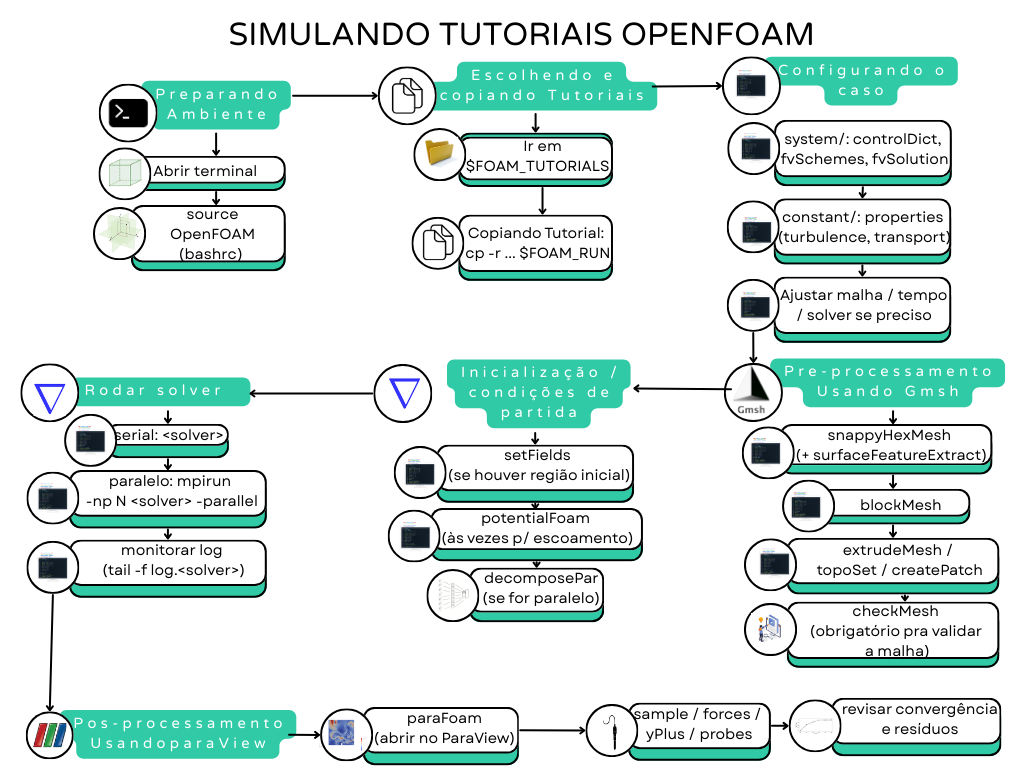
\includegraphics[width=.72\textwidth]{fluxograma_openfoam.png}
\caption{Fluxo de trabalho para preparação dos casos e pós-processamento no OpenFOAM, empregado no relatório parcial e no artigo do CBCFD.}\label{fig:fluxo}
\end{figure}

A Tabela~\ref{tab:etapas} confronta o cronograma aprovado com a execução documentada. O termo ``parcial'' indica que houve avanço verificável, mas não conclusão de toda a abrangência originalmente proposta.

\begin{table}[H]\centering\caption{Alinhamento entre etapas do plano de trabalho e execução final.}\label{tab:etapas}\scriptsize
\begin{tabularx}{\textwidth}{p{2.25cm}p{2.45cm}X p{1.45cm}}\toprule
Período previsto&Etapa&Execução e evidência&Situação\\\midrule
Mês 1&Revisão inicial&CFD, turbulência, OpenFOAM, POD, autoencoders e SINDy; referências incorporadas ao relatório parcial e ao presente texto.&Concluída\\
Meses 2--4&Formação e tutoriais&Casos pitzDaily, damBreakLaminarFine, movingCone e aerofoil; prática com malha, dicionários, execução e ParaView.&Concluída\\
Meses 5--7&Simulação e dados&Casos simplificados cavity e dam-break; padronização de snapshots; primeiros POD e SAE; entrega do relatório parcial.&Concluída\\
Meses 8--9&Modelos reduzidos&Comparação POD/SAE e ampliação progressiva para os regimes laminar, URANS e LES.&Concluída\\
Meses 10--11&Identificação e interpretação&POD--SINDy, SAE--SINDy e SAE--POD--SINDy; integração livre, auditoria de proveniência e validação direta da cavity.&Concluída\\
Meses 10--11&Análise paramétrica&Comparação qualitativa dos fechamentos laminar, SST e WALE; sem varredura controlada de Reynolds, geometria ou condições de contorno.&Parcial\\
Meses 8--11&Substituto no OpenFOAM&Equações reduzidas identificadas e campos reconstruídos, mas sem implementação de um novo modelo/solver validado no OpenFOAM.&Parcial\\
Mês 12&Relatório e divulgação&Quatro relatórios técnicos, relatório final consolidado e artigo de congresso.&Concluída\\\bottomrule
\end{tabularx}\end{table}

Essa sequência também explica a mudança de escala dos dados. O artigo do CBCFD documenta uma prova de conceito da cavity com 1001 snapshots e estado formado apenas por $U_x,U_y$. A análise final não substitui retroativamente aquele experimento: ela amplia e audita o caso, usando 5645 snapshots válidos e $U_x,U_y,p,T,k$. Por isso, as métricas das duas etapas são apresentadas separadamente.

\subsection{Casos OpenFOAM}
A Tabela~\ref{tab:casos} alinha as configurações centrais. Os casos dam-break têm 2268 células e duração de 1 s; a cavidade tem 1600 células e duração de 5 s. Os dicionários \texttt{controlDict}, \texttt{fvSchemes}, \texttt{fvSolution}, transporte e propriedades foram auditados diretamente.

\begin{table}[H]\centering\caption{Casos de alta fidelidade analisados.}\label{tab:casos}\scriptsize
\begin{tabularx}{\textwidth}{lXXXX}\toprule
Caso&Solver/modelo&Malha&Tempo&Observações\\\midrule
Dam-break laminar&\texttt{incompressibleVoF}, laminar&2268, quase 2D&0--1 s; $\Delta t=10^{-4}$&10001 saídas\\
Dam-break URANS&\texttt{incompressibleVoF}, SST&2268, quase 2D&0--1 s; $\Delta t=10^{-4}$&10001 saídas\\
Dam-break LES&\texttt{incompressibleVoF}, WALE&2268, quase 2D&0--1 s; $\Delta t=10^{-4}$&1001 saídas; gravação a cada $10^{-3}$ s\\
Cavity URANS&\texttt{fluid}, gás perfeito, SST&$40\times40\times1$&0--5 s; $\Delta t=5\times10^{-4}$&5646 diretórios presentes\\\bottomrule
\end{tabularx}\end{table}

Todos empregam Euler de primeira ordem no tempo. Os dam-break usam PIMPLE e MULES; a cavidade usa PIMPLE com tampa a $1\,\mathrm{m\,s^{-1}}$. A ausência de adaptação efetiva do passo e de estudos de independência de malha constitui limitação comum.

No LES--WALE, a contagem foi verificada diretamente: existem 1001 diretórios temporais, de $t=0$ a 1 s, uniformemente separados por $10^{-3}$ s. O \texttt{controlDict} usa $\Delta t=10^{-4}$ s e \texttt{writeInterval}=0,001 s; portanto, são executados aproximadamente 10000 passos numéricos e armazenados 1001 estados, incluindo os extremos. Não ocorreu redução posterior de 10001 para 1001 snapshots na POD: os arquivos POD e POD--SINDy contêm todos os 1001 tempos. A subamostragem adicional ocorreu somente na cadeia SAE legada, que usou \texttt{stride}=10 e 101 estados; o SAE corrigido usa \texttt{stride}=1, isto é, os 1001 snapshots disponíveis.

\subsection{Redução POD e SAE}
A POD seguiu as Equações~\eqref{eq:matriz_snapshots}--\eqref{eq:pod_metricas}. Cada coluna reuniu os canais físicos de um tempo; após subtrair a média temporal, a SVD forneceu modos, coeficientes e energia. Os resultados são apresentados por $E_r$ e $\varepsilon_{\mathrm{POD}}$. Na cavidade, a auditoria motivou nova execução: os canais legados $\alpha_{water}$ e $p_{rgh}$ foram substituídos por $p$ e $T$, e a normalização individual de cada snapshot foi removida, pois a transformação $x_i\mapsto x_i/\lVert x_i\rVert_2$ destruiria a informação de amplitude necessária à reconstrução física.

Os autoencoders usam divisão temporal, sem mistura entre passado de treino e futuro de validação, e normalização pela Equação~\eqref{eq:normalizacao_sae}. As dimensões latentes variaram de quatro a 32. A execução corrigida do LES usou camadas $11520\!\rightarrow512\!\rightarrow256\!\rightarrow128\!\rightarrow32$ no encoder e estrutura simétrica no decoder, Adam, perda Huber e $\lambda_z=0$. Para cada snapshot foram calculados
\begin{equation}
\operatorname{MSE}_i=\frac{1}{n}\lVert x_i-\widehat x_i\rVert_2^2,
\qquad
\varepsilon_i=\frac{\lVert x_i-\widehat x_i\rVert_2}{\lVert x_i\rVert_2+\epsilon},
\label{eq:metricas_snapshot}
\end{equation}
e, sobre todo o conjunto,
\begin{equation}
R^2=1-\frac{\sum_i\lVert x_i-\widehat x_i\rVert_2^2}
{\sum_i\lVert x_i-\bar x\rVert_2^2}.
\label{eq:r2}
\end{equation}
Os artefatos efetivamente salvos foram priorizados sobre configurações apenas declaradas nos notebooks. No LES, distinguem-se o SAE legado, com 101 tempos e oito latentes, usado pelos SINDy salvos, e o SAE corrigido, com 1001 tempos e 32 latentes.

\subsection{Identificação e avaliação dinâmica}
Foram avaliados:
\begin{enumerate}
\item \textbf{POD--SINDy}: $q(t)=a(t)$ da Equação~\eqref{eq:pod_projecao};
\item \textbf{SAE--SINDy}: $q(t)=z(t)=f_\theta(\widetilde x(t))$;
\item \textbf{SAE--POD--SINDy}: $q(t)$ obtido pela Equação~\eqref{eq:pod_latente}, seguido da reconstrução da Equação~\eqref{eq:decodificacao_hibrida}.
\end{enumerate}
Após estimar $\dot Q$, os coeficientes foram ajustados conforme as Equações~\eqref{eq:sindy} e \eqref{eq:alasso}. O erro relativo das derivadas é
\begin{equation}
\varepsilon_{\dot q}=\frac{\lVert\dot Q-\Theta(Q,t)\widehat\Xi\rVert_F}{\lVert\dot Q\rVert_F}.
\label{eq:erro_derivada}
\end{equation}
Para uma trajetória de referência $Q$ e uma previsão $\widehat Q$, usaram-se
\begin{equation}
\varepsilon_{\mathrm{traj}}=\frac{\lVert Q-\widehat Q\rVert_F}{\lVert Q\rVert_F},
\qquad
R^2_{\mathrm{traj}}=1-\frac{\lVert Q-\widehat Q\rVert_F^2}{\lVert Q-\bar Q\rVert_F^2}.
\label{eq:metricas_trajetoria}
\end{equation}
Também foram registrados erro de um passo e número de coeficientes não nulos. Na previsão de um passo, pode-se escrever esquematicamente $\widehat q_{i+1}=q_i+\Delta t\,\Theta(q_i,t_i)\widehat\Xi$; como $q_i$ é verdadeiro a cada reinício, o erro não acumula. Já a trajetória livre resulta da integração contínua da Equação~\eqref{eq:integracao_livre}. Resultados de fallback guiado foram, portanto, explicitamente separados de previsão autônoma.

\subsection{Auditoria e alinhamento}
Foram comparados caminhos internos, hashes, dimensões, canais e tempos dos NPZ, Keras e JSON. A similaridade superior a 99\% entre notebooks de casos diferentes confirmou reutilização de templates. Isso é aceitável apenas quando campos e hipóteses são adaptados. Na cavidade foi criado um validador que lê $U,p,T,k$ diretamente do OpenFOAM e associa cada estado SINDy ao tempo físico mais próximo.

\novasecao{RESULTADOS E DISCUSSÃO}
\subsection{Evolução desde o relatório parcial e o artigo do CBCFD}
O relatório parcial, referente ao período de 30/10/2025 a 28/02/2026, registrou a conclusão da revisão e da formação nas ferramentas e a fase final de geração dos primeiros dados. Tratava-se ainda de conjuntos exploratórios: a cavity preliminar tinha malha $120\times120\times1$ e somente 11 snapshots entre 0 e 1 s; o damBreakLaminarFine tinha cerca de 7700 células e 21 snapshots. Naquele momento, a POD já fornecia coeficientes regulares para a cavity, enquanto os SAE iniciais apresentavam sobreajuste ou subajuste. Esse diagnóstico orientou aumento do número de snapshots, revisão da normalização, ajuste de dimensão latente e separação temporal de treino e validação.

A etapa seguinte gerou o artigo \textit{Redução de dimensionalidade em escoamento cavity via POD e SAE a partir de dados do OpenFOAM}, de Eldo Francisco Chagas Junior e Daniela de Oliveira Maionchi, publicado no congresso CBCFD. Nesse recorte, foram usados 1001 snapshots uniformes, $0\leq t\leq5$ s e $\Delta t=0,005$ s, em uma malha de 1600 células. O vetor continha somente $U_x$ e $U_y$, totalizando 3200 variáveis. A POD concentrou 68,59\% da energia no primeiro modo, 95\% em cinco modos e 99\% em nove. O SAE com 16 latentes obteve $R^2=0,9954$ no treino e 0,9934 na validação, erro relativo médio de validação 0,0801 e menor perda de validação 0,0045. O artigo cumpriu a meta de comparar redução linear e não linear e deixou SINDy explicitamente como continuidade.

A etapa final executou essa continuidade e tornou o teste mais exigente: adicionou campos termodinâmicos e turbulentos, comparou quatro regimes e avaliou previsão autônoma. Os resultados posteriores da cavity não devem ser confrontados diretamente com os números do artigo como se fossem a mesma experiência. O conjunto final possui mais tempos, cinco canais, outro pré-processamento e uma divisão temporal distinta. A redução do $R^2$ do SAE final para 0,825 reflete, entre outros fatores, esse aumento da dimensionalidade física e o protocolo mais rigoroso, não uma correção dos resultados publicados.

\subsection{Representação por POD}
A Tabela~\ref{tab:pod} mostra que 50 modos representam bem todos os conjuntos, mas há ressalvas de proveniência. No dam-break laminar e no LES, $k$ foi solicitado embora ausente e substituído por zero; no URANS salvo, a POD efetiva contém somente velocidade. Na cavidade, apresentam-se os números da execução corrigida.

\begin{table}[H]\centering\caption{Síntese dos resultados POD com 50 modos.}\label{tab:pod}
\begin{tabular}{lccc}\toprule Caso&Snapshots&Energia&Erro relativo\\\midrule
Dam-break laminar&10001&0,9962&0,0617\\
Dam-break URANS&10001&0,9936&0,0802\\
Dam-break LES--WALE&1001&0,9936&0,0800\\
Cavity corrigida&5645&0,99988&0,01083\\\bottomrule
\end{tabular}\end{table}

\begin{figure}[H]\centering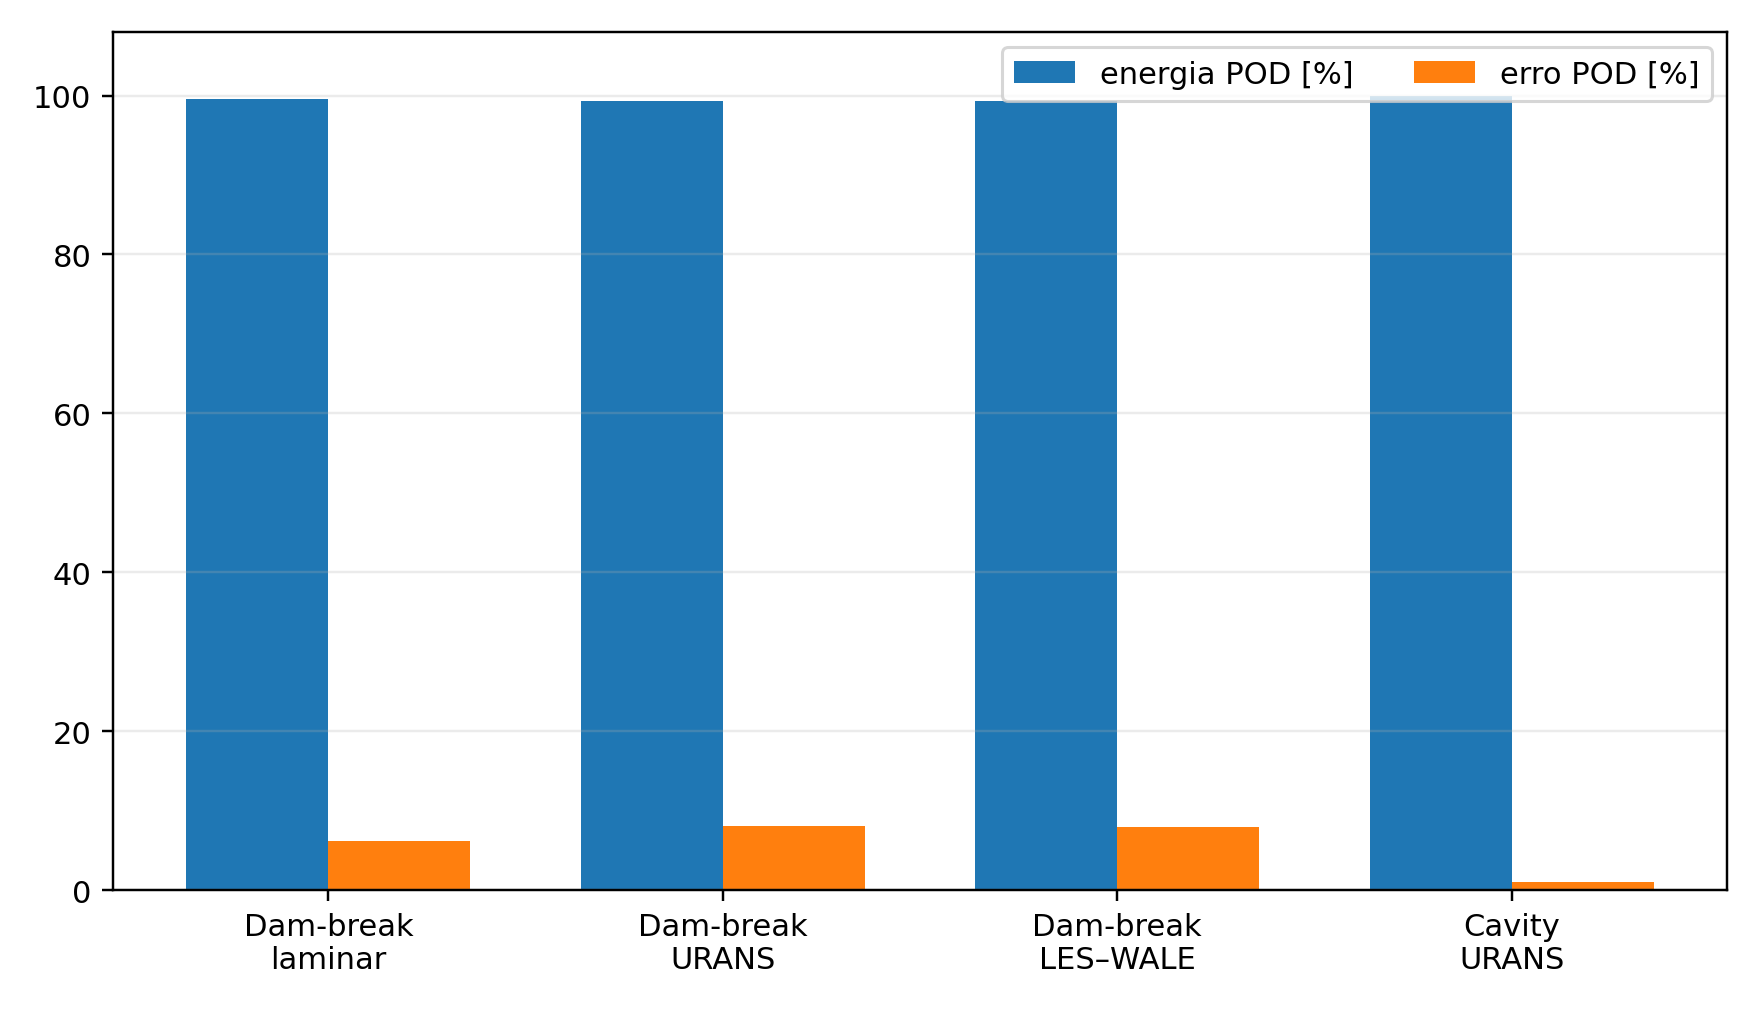
\includegraphics[width=.78\textwidth]{comparacao_pod.png}\caption{Energia e erro POD. Na cavidade usa-se a reexecução corrigida; nos dam-break permanecem as ressalvas de canais.}\end{figure}

A POD é, portanto, eficiente para reconstrução. Isso não garante dinâmica: nos modelos SINDy, pequenas componentes e derivadas podem ser decisivas mesmo quando sua contribuição energética é baixa. A Figura~\ref{fig:modos} ilustra modos dominantes de dois casos.

\begin{figure}[H]\centering
\begin{subfigure}{.48\textwidth}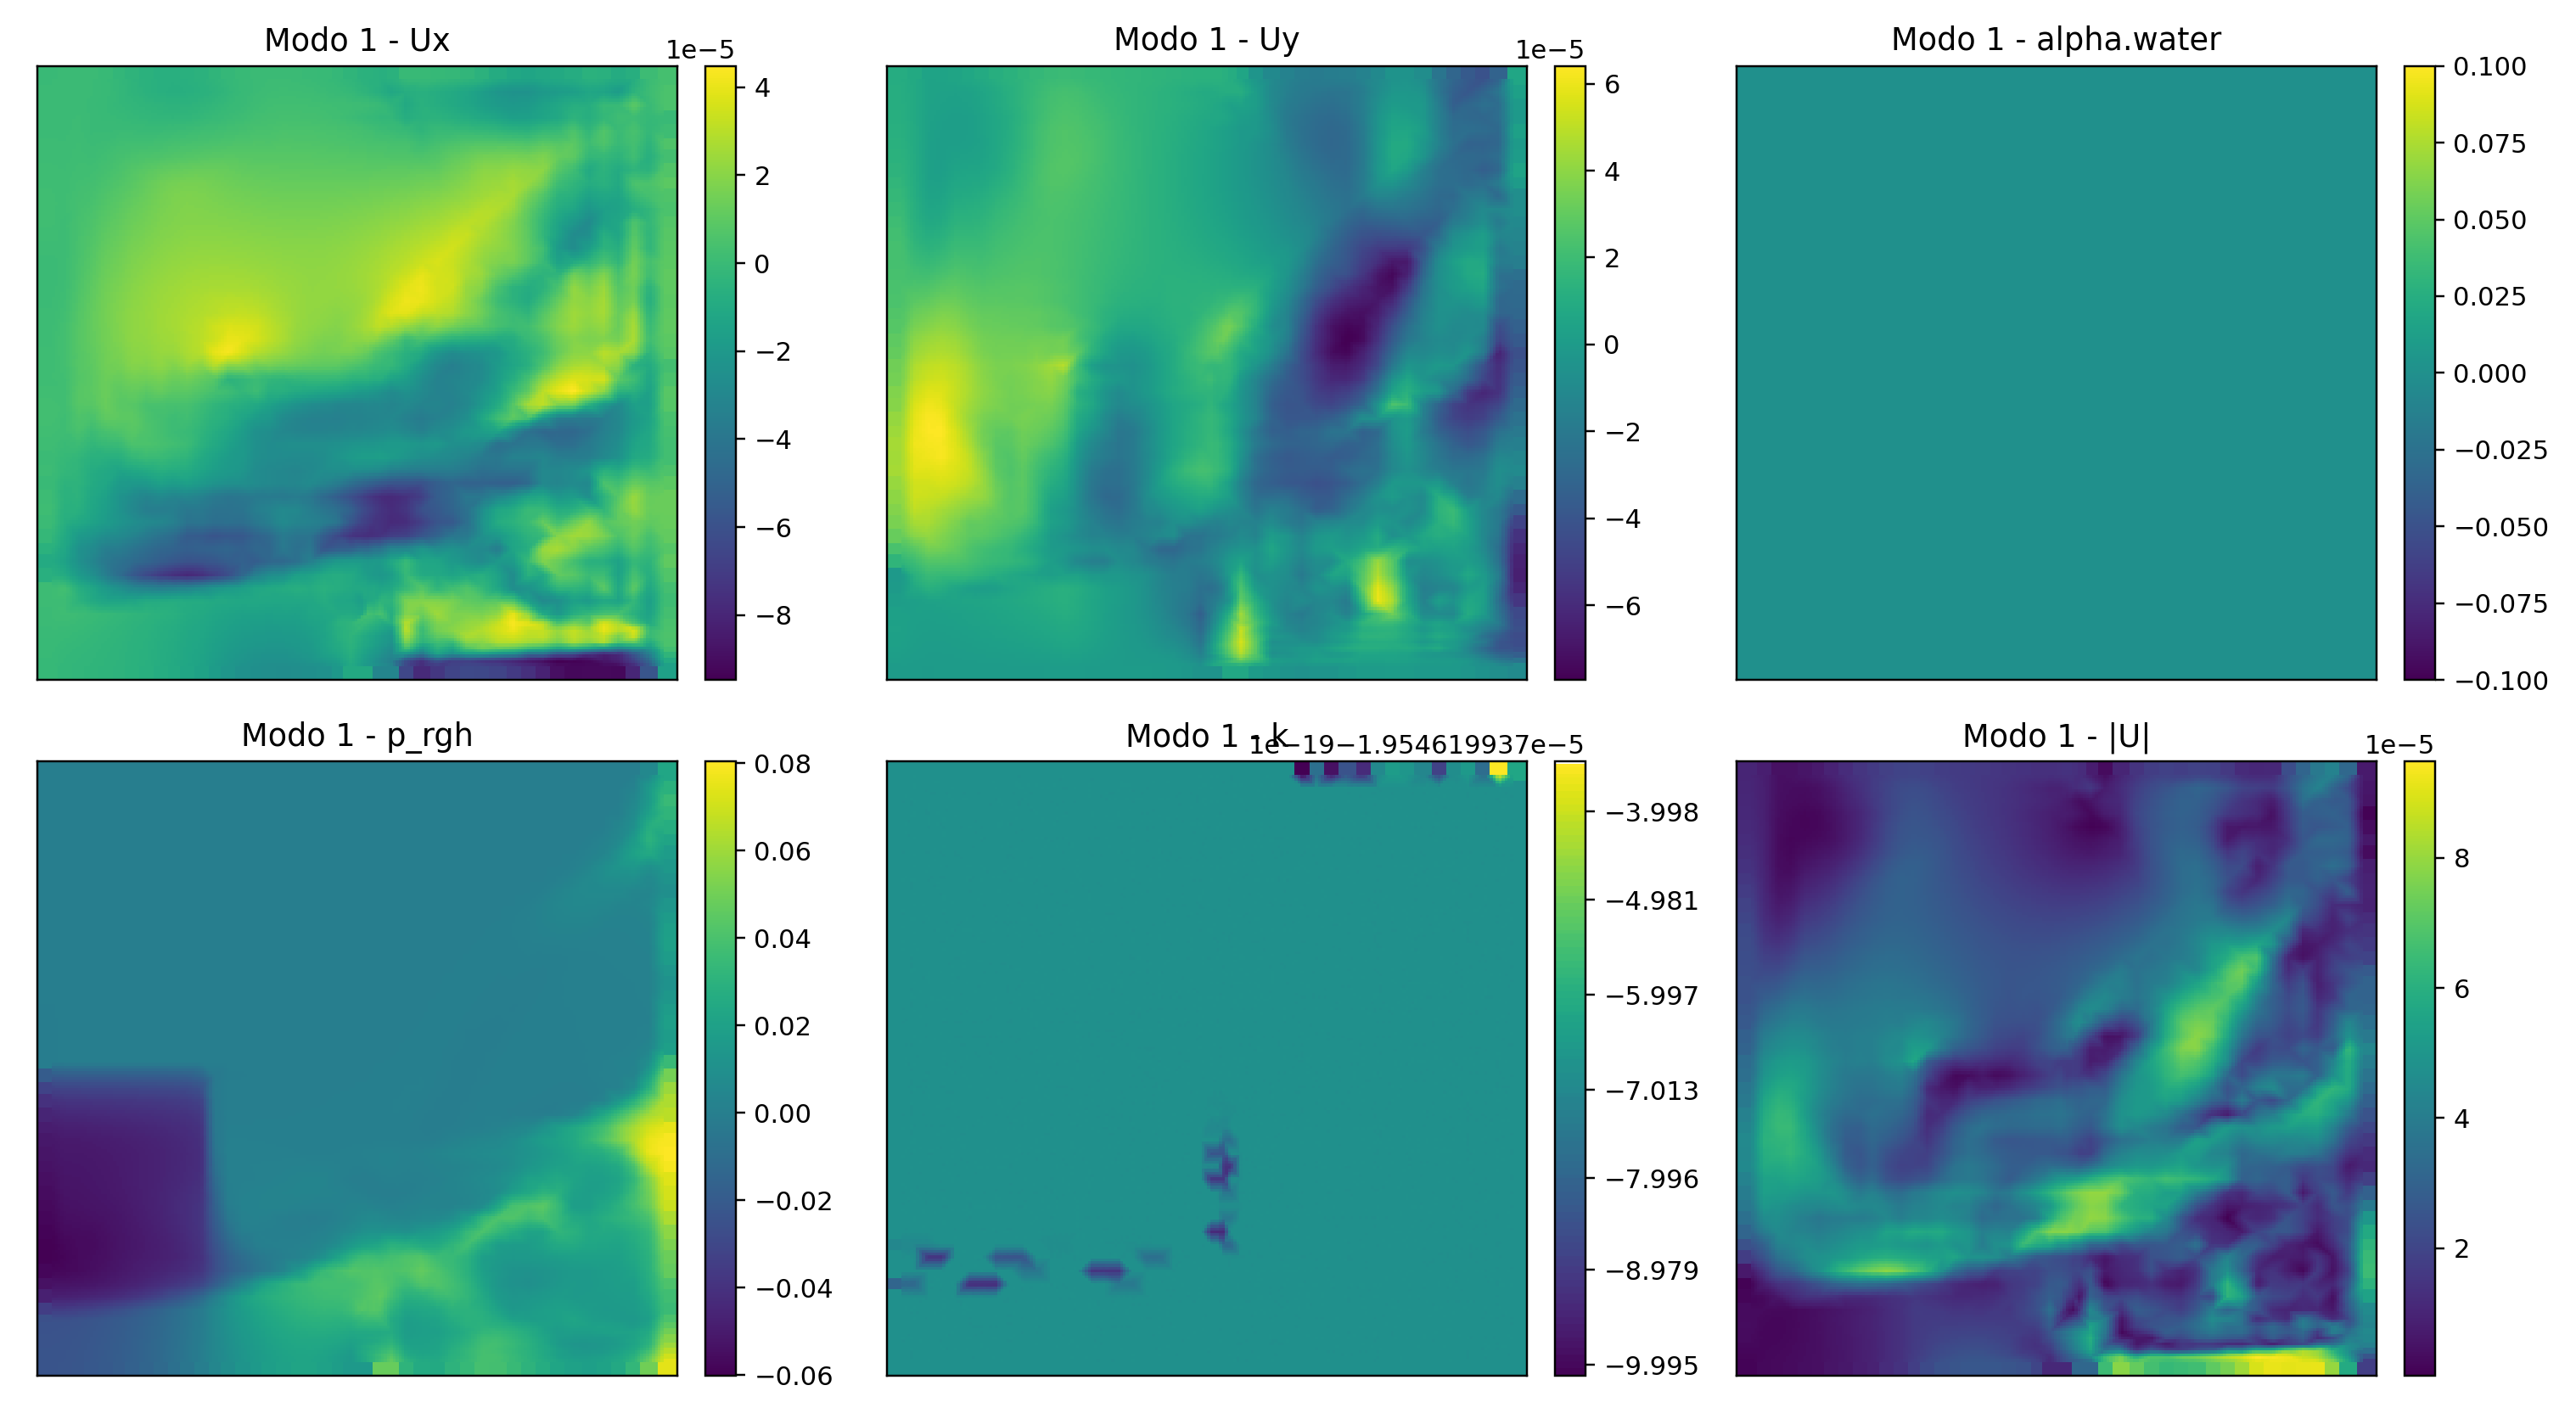
\includegraphics[width=\linewidth]{les_pod_modo1.png}\caption{LES--WALE.}\end{subfigure}\hfill
\begin{subfigure}{.48\textwidth}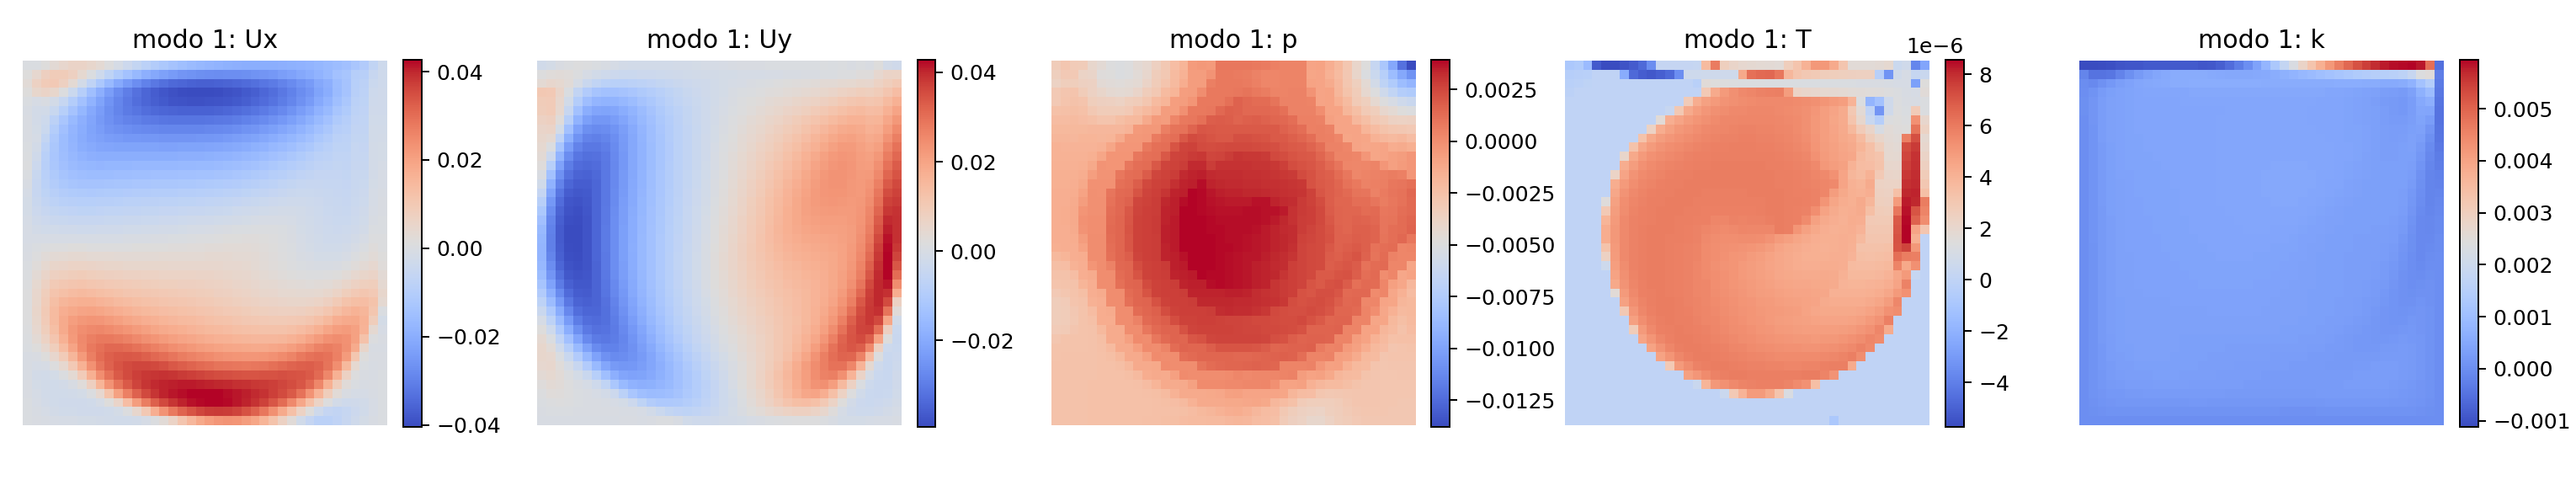
\includegraphics[width=\linewidth]{cavity_pod_modo1.png}\caption{Cavity corrigida.}\end{subfigure}
\caption{Primeiro modo POD multivariável.}\label{fig:modos}\end{figure}

\subsection{Representação por SAE}
O SAE não foi uniformemente superior à POD. O URANS dam-break apresentou a melhor generalização, enquanto os dois outros dam-break tiveram grande diferença entre treino e validação. No LES, a correção elevou $R^2_{treino}$ de 0,585 para 0,989, mas $R^2_{val}$ permaneceu 0,263. Isso caracteriza boa representação dos snapshots vistos e extrapolação temporal limitada.

\begin{table}[H]\centering\caption{Síntese dos SAE usados ou corrigidos.}\label{tab:sae}
\begin{tabular}{lcccc}\toprule Caso&Latentes&$R^2_{treino}$&$R^2_{val}$&Erro $L_2$ val.\\\midrule
Dam-break laminar&8&0,822&0,133&0,918\\
Dam-break URANS&4&0,949&0,942&0,241\\
Dam-break LES corrigido&32&0,989&0,263&0,814\\
Cavity&8&0,809&0,825&0,392\\\bottomrule
\end{tabular}\end{table}

\begin{figure}[H]\centering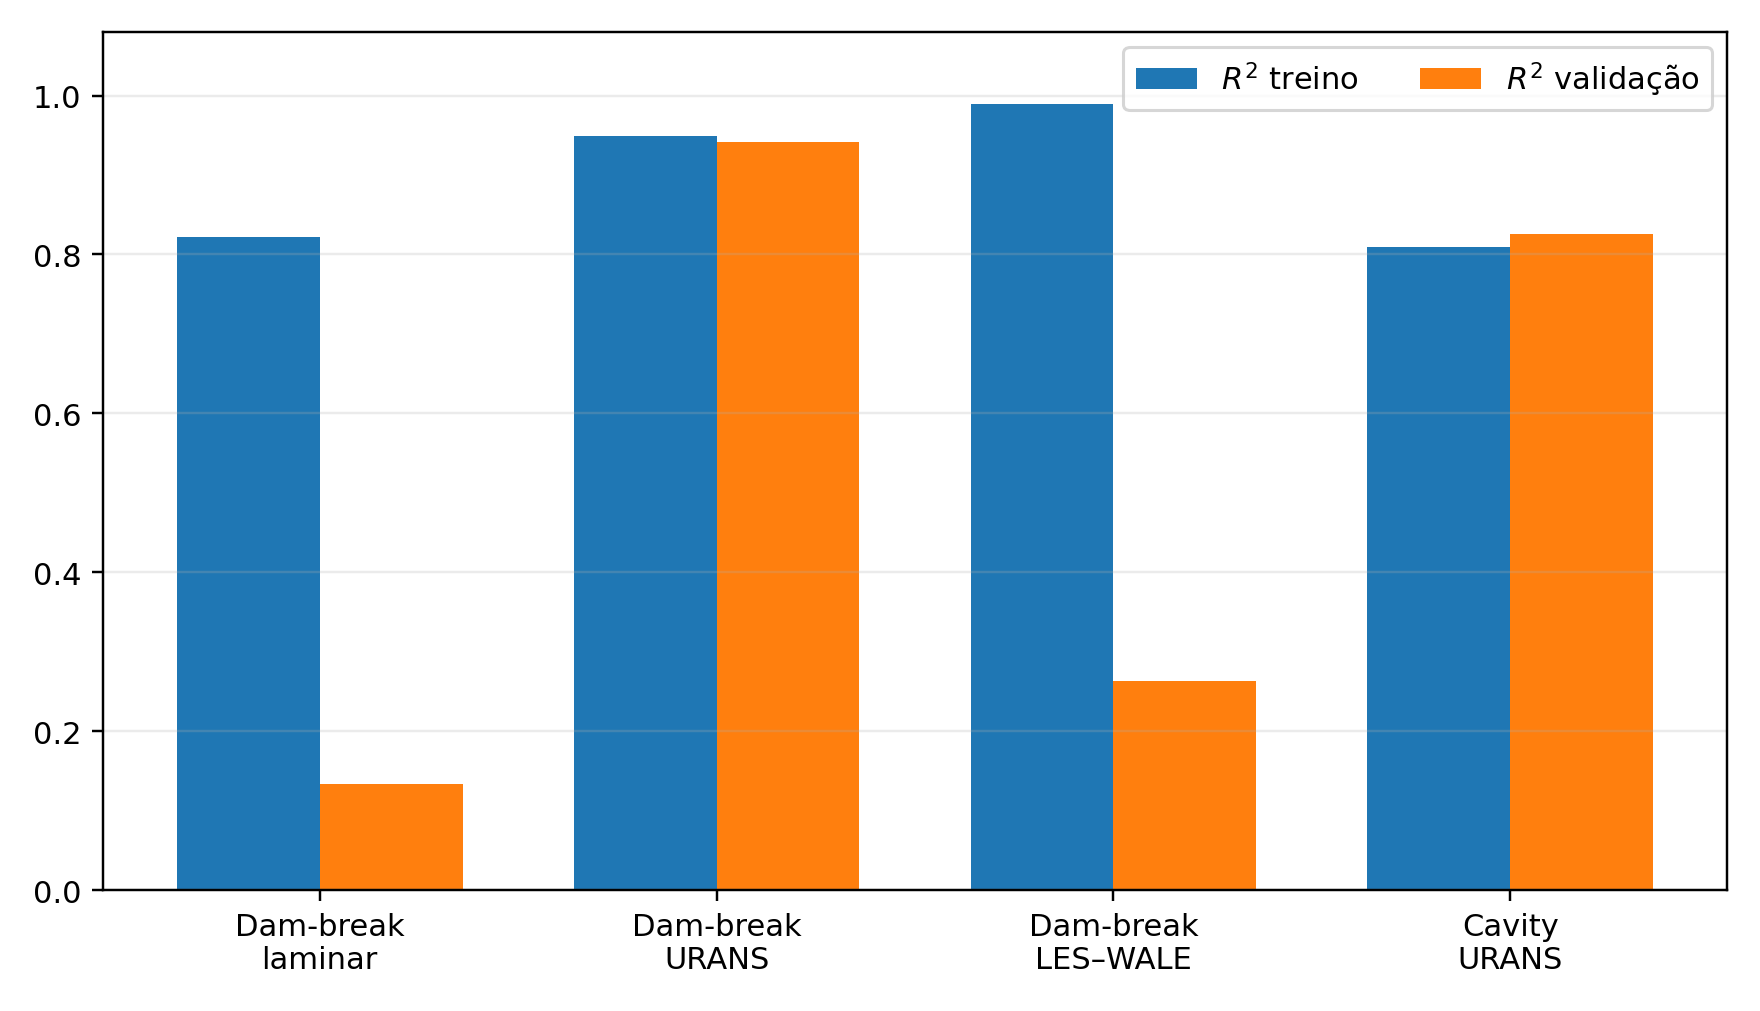
\includegraphics[width=.78\textwidth]{comparacao_sae.png}\caption{Comparação do $R^2$ de reconstrução dos SAE. O LES corresponde à configuração corrigida; seus SINDy salvos ainda usam o latente antigo.}\end{figure}

A vantagem teórica da variedade não linear depende de arquitetura, quantidade de dados, normalização e objetivo de treinamento. Minimizar apenas reconstrução não força suavidade temporal nem fechamento dinâmico.

\subsection{Dinâmica identificada por SINDy}
Os modelos diretos foram frágeis. POD--SINDy falhou em integração livre nos casos laminar, URANS e cavity corrigida; no LES integrou, mas com erro 1,652. SAE--SINDy falhou em todos os casos, apesar de erros guiados por vezes pequenos. Esses resultados confirmam que avaliação de derivadas ou de um passo não basta.

\begin{table}[H]\centering\caption{Comparação dinâmica dos modelos SINDy.}\label{tab:sindy}\small
\begin{tabularx}{\textwidth}{lcccX}\toprule
Caso&POD--SINDy&SAE--SINDy&SAE--POD--SINDy&Interpretação\\\midrule
Laminar&livre falha&livre falha&erro 0,634; $R^2=0,598$&POD latente estabiliza, sem alta precisão\\
URANS&livre falha&livre falha&erro 0,551; $R^2=0,697$&melhor resultado global\\
LES--WALE&erro 1,652&livre falha&erro 0,858; $R^2=0,264$&estável, porém baixa fidelidade\\
Cavity&livre falha&livre falha&erro 0,644; $R^2=0,586$&campos diretos razoáveis, piora no final\\\bottomrule
\end{tabularx}\end{table}

\begin{figure}[H]\centering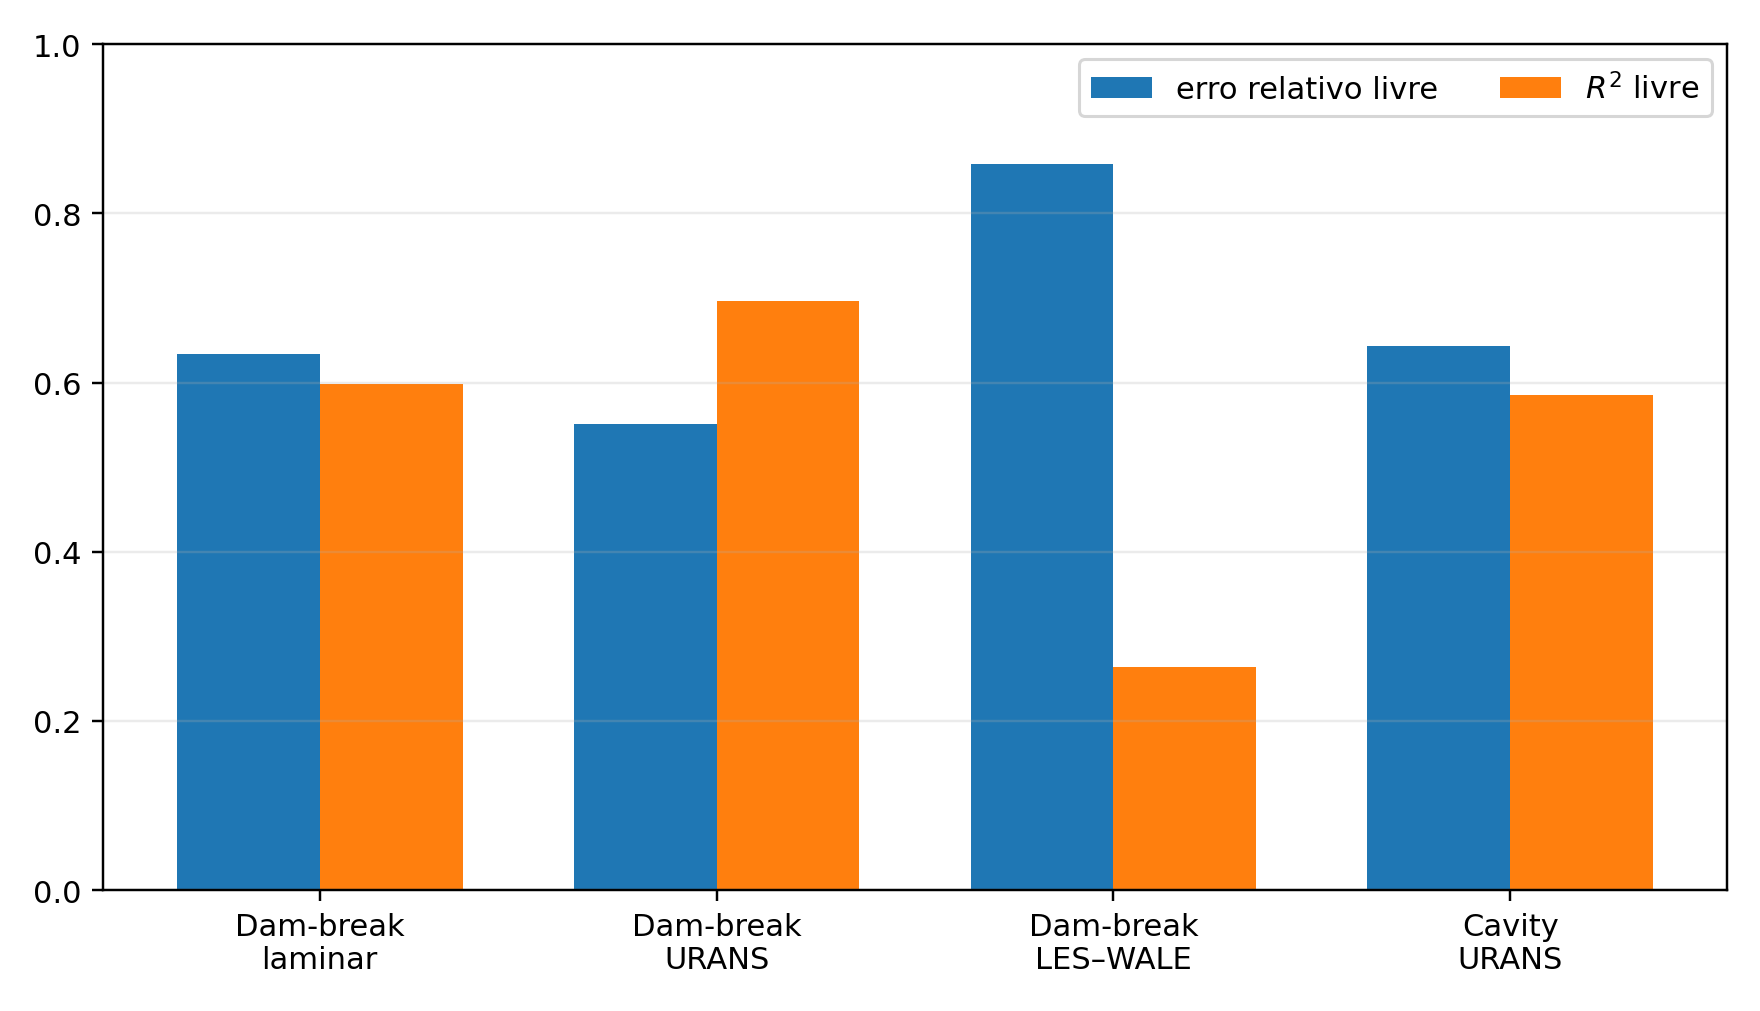
\includegraphics[width=.78\textwidth]{comparacao_hibrido.png}\caption{Erro relativo e $R^2$ da integração livre SAE--POD--SINDy.}\end{figure}

\subsection{POD como estabilizador latente}
O híbrido foi o único arranjo que completou integração livre nos quatro casos. A energia preservada pela POD latente foi 90,95\% no laminar, praticamente 100\% no URANS, 88,45\% no LES e 96,68\% na cavity. No URANS, a POD é equidimensional, aproximando a recomendação de Lin, Xiao e Fang \cite{lin2024}; nos demais casos há truncamento e, portanto, estabilização e filtragem ocorrem simultaneamente.

O ganho deve ser interpretado com cautela. No laminar, todos os 32 coeficientes possíveis foram mantidos; no cavity, o modelo é mais esparso, com 11 de 40 termos. O LES tem o melhor ajuste local de derivadas, erro 0,187, mas o pior $R^2$ livre. Logo, bom ajuste local não determina estabilidade ou generalização global.

\begin{figure}[H]\centering
\begin{subfigure}{.49\textwidth}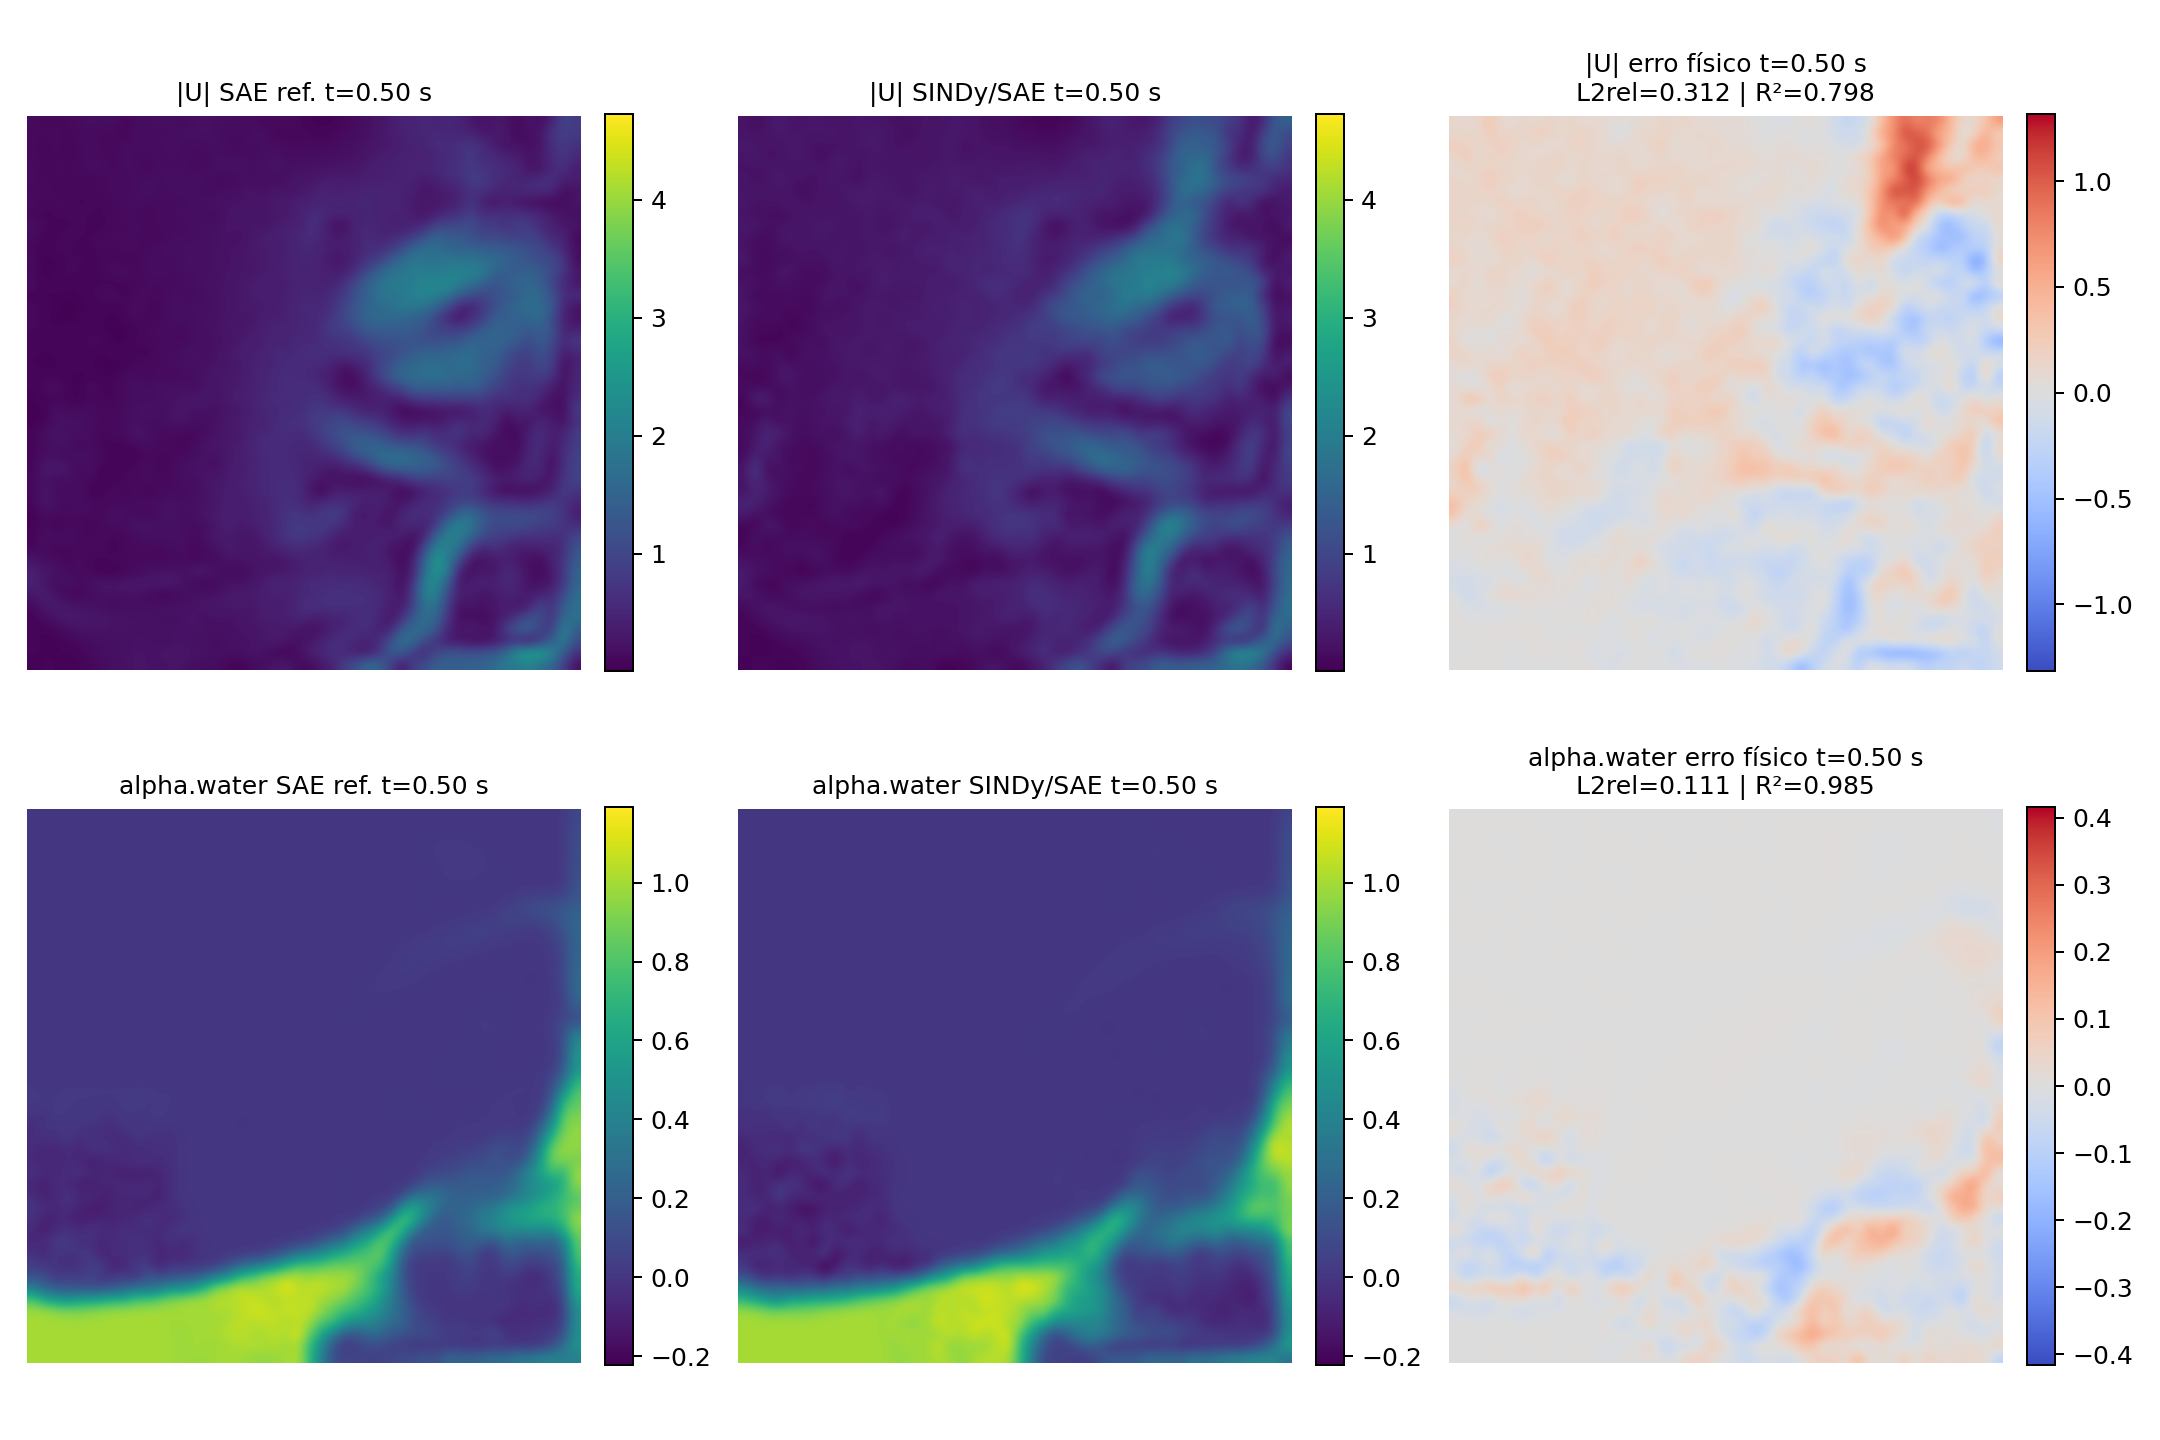
\includegraphics[width=\linewidth]{laminar_hibrido.png}\caption{Dam-break laminar.}\end{subfigure}\hfill
\begin{subfigure}{.49\textwidth}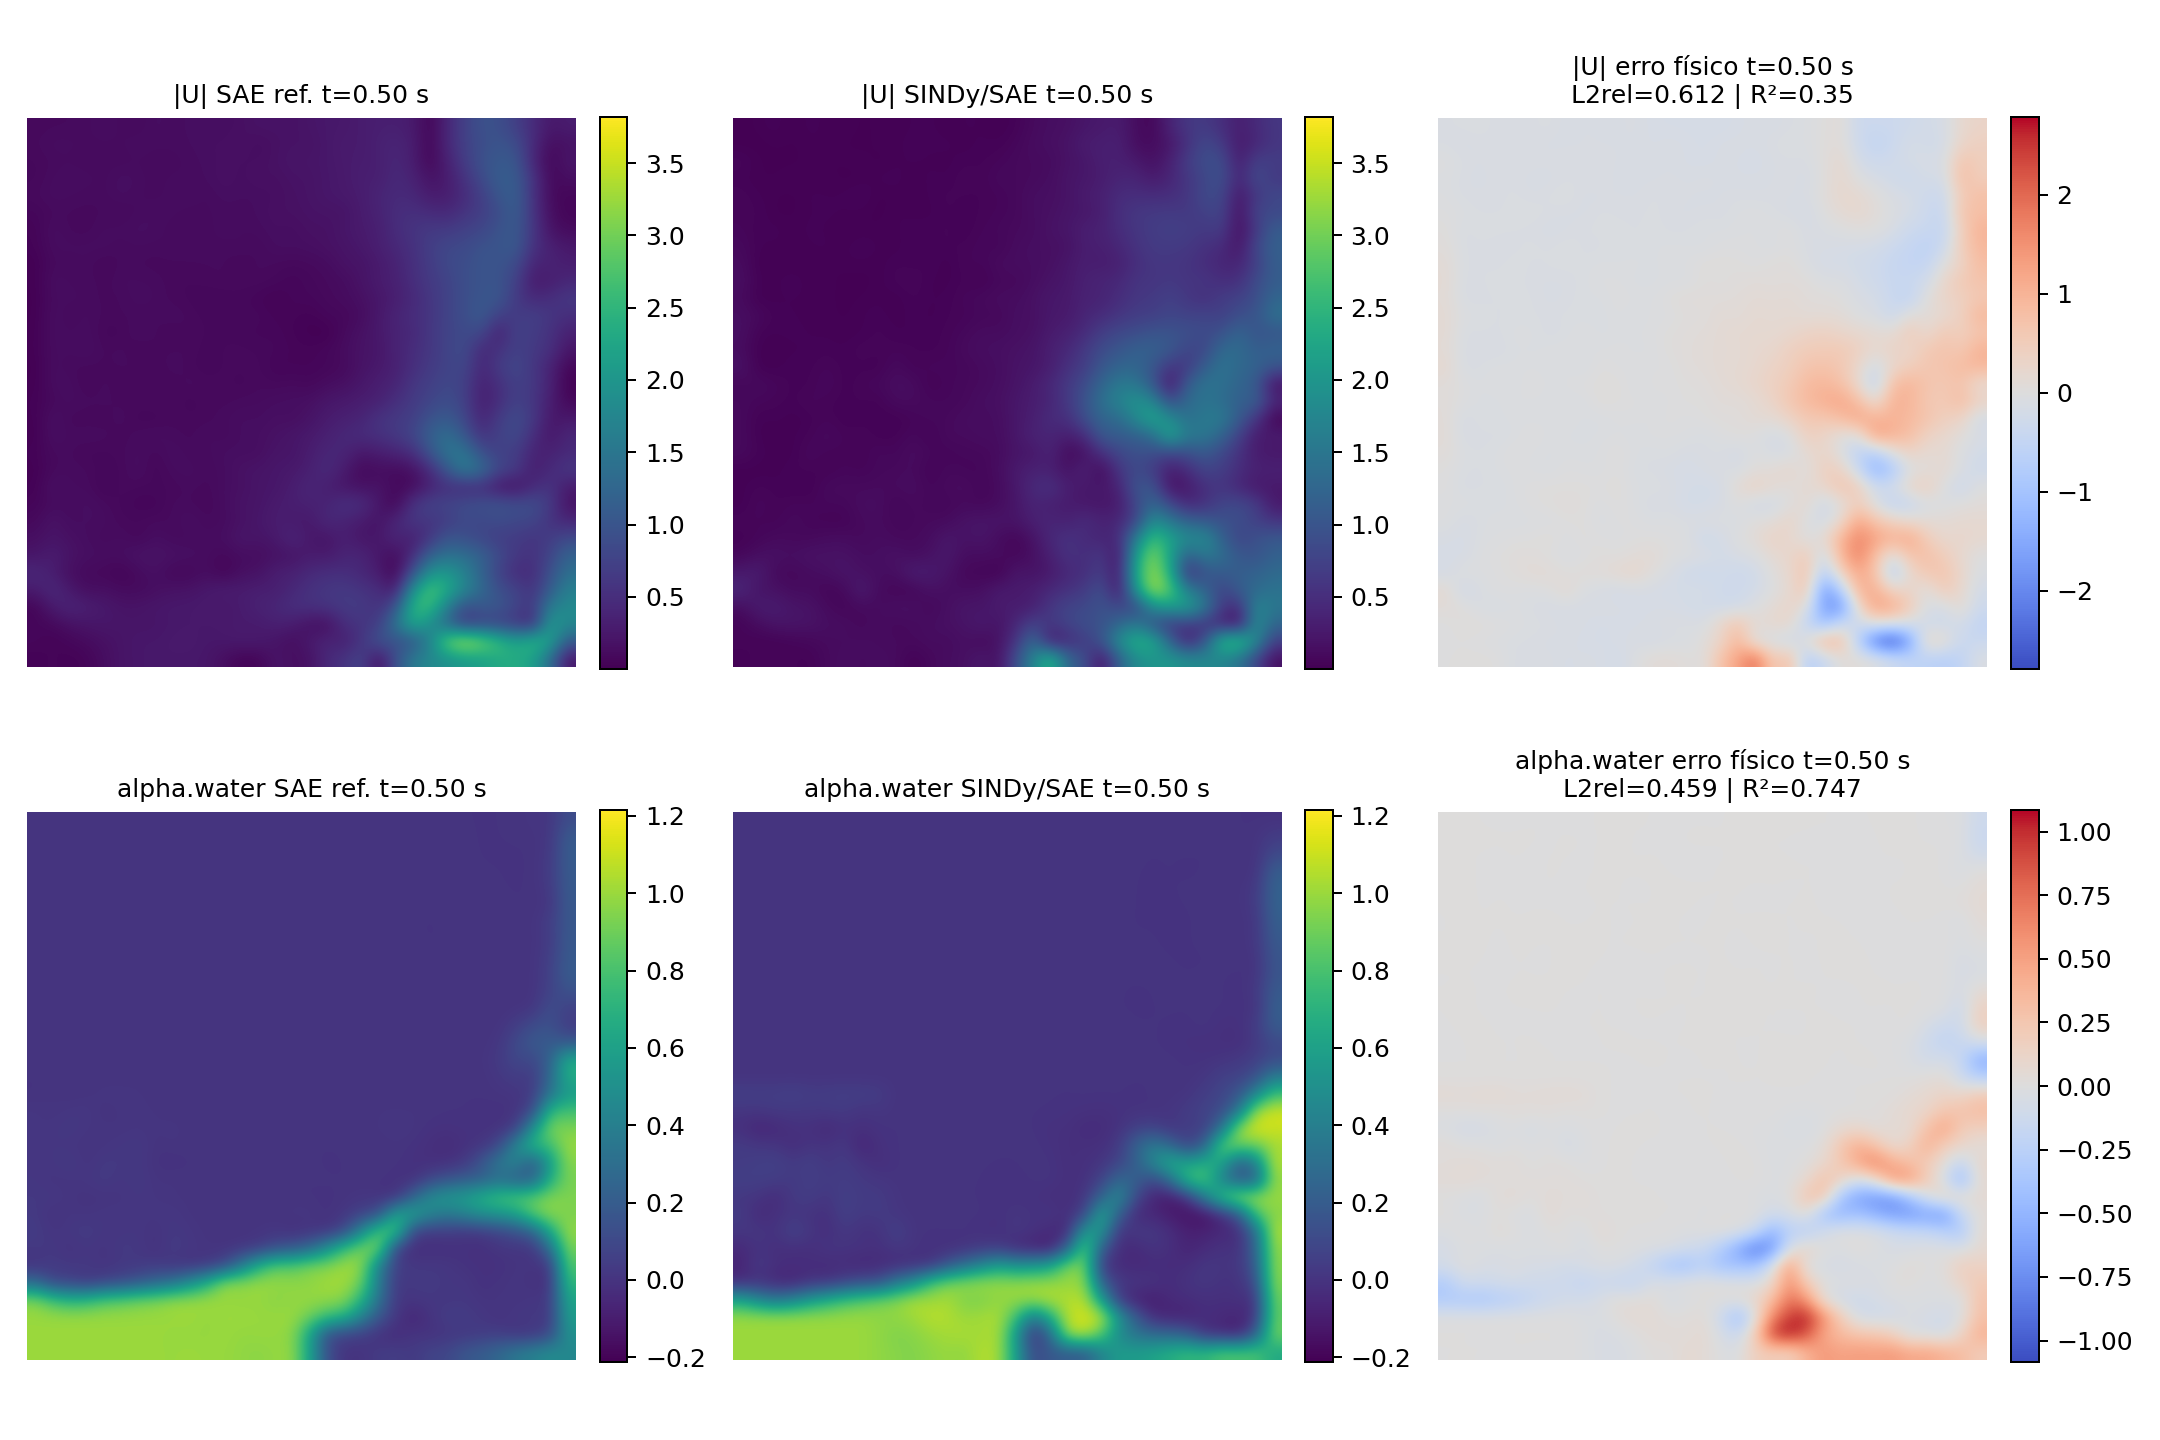
\includegraphics[width=\linewidth]{urans_hibrido.png}\caption{Dam-break URANS.}\end{subfigure}
\caption{Campos decodificados pela integração livre do modelo híbrido.}\end{figure}

\begin{figure}[H]\centering
\begin{subfigure}{.49\textwidth}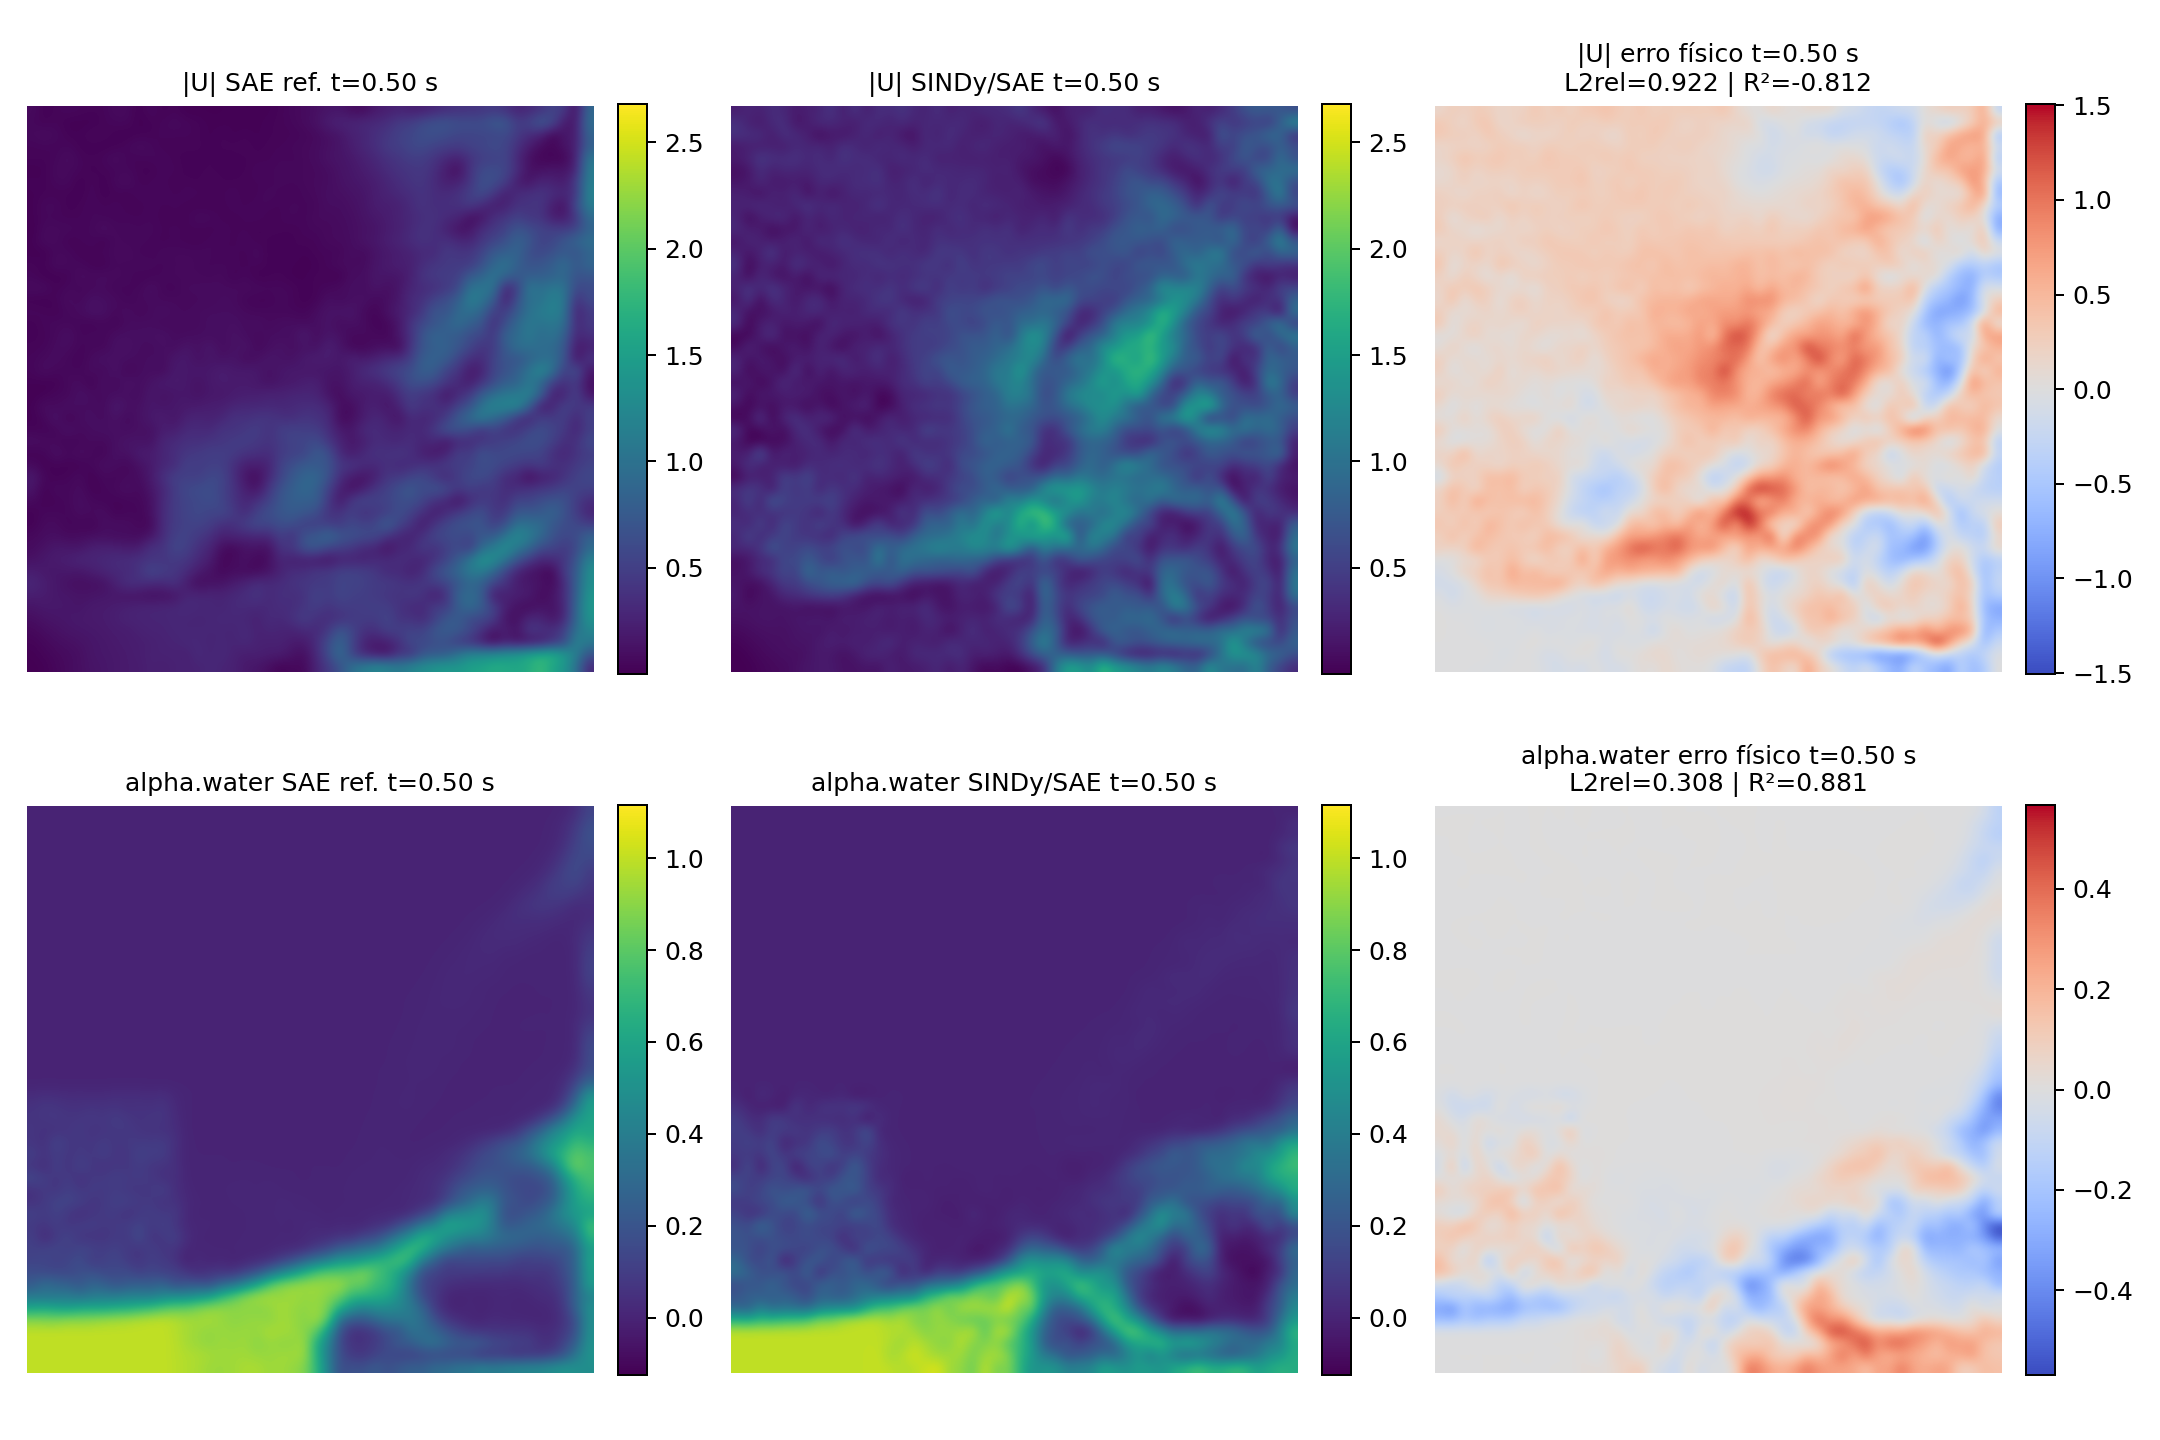
\includegraphics[width=\linewidth]{les_hibrido.png}\caption{Dam-break LES--WALE.}\end{subfigure}\hfill
\begin{subfigure}{.49\textwidth}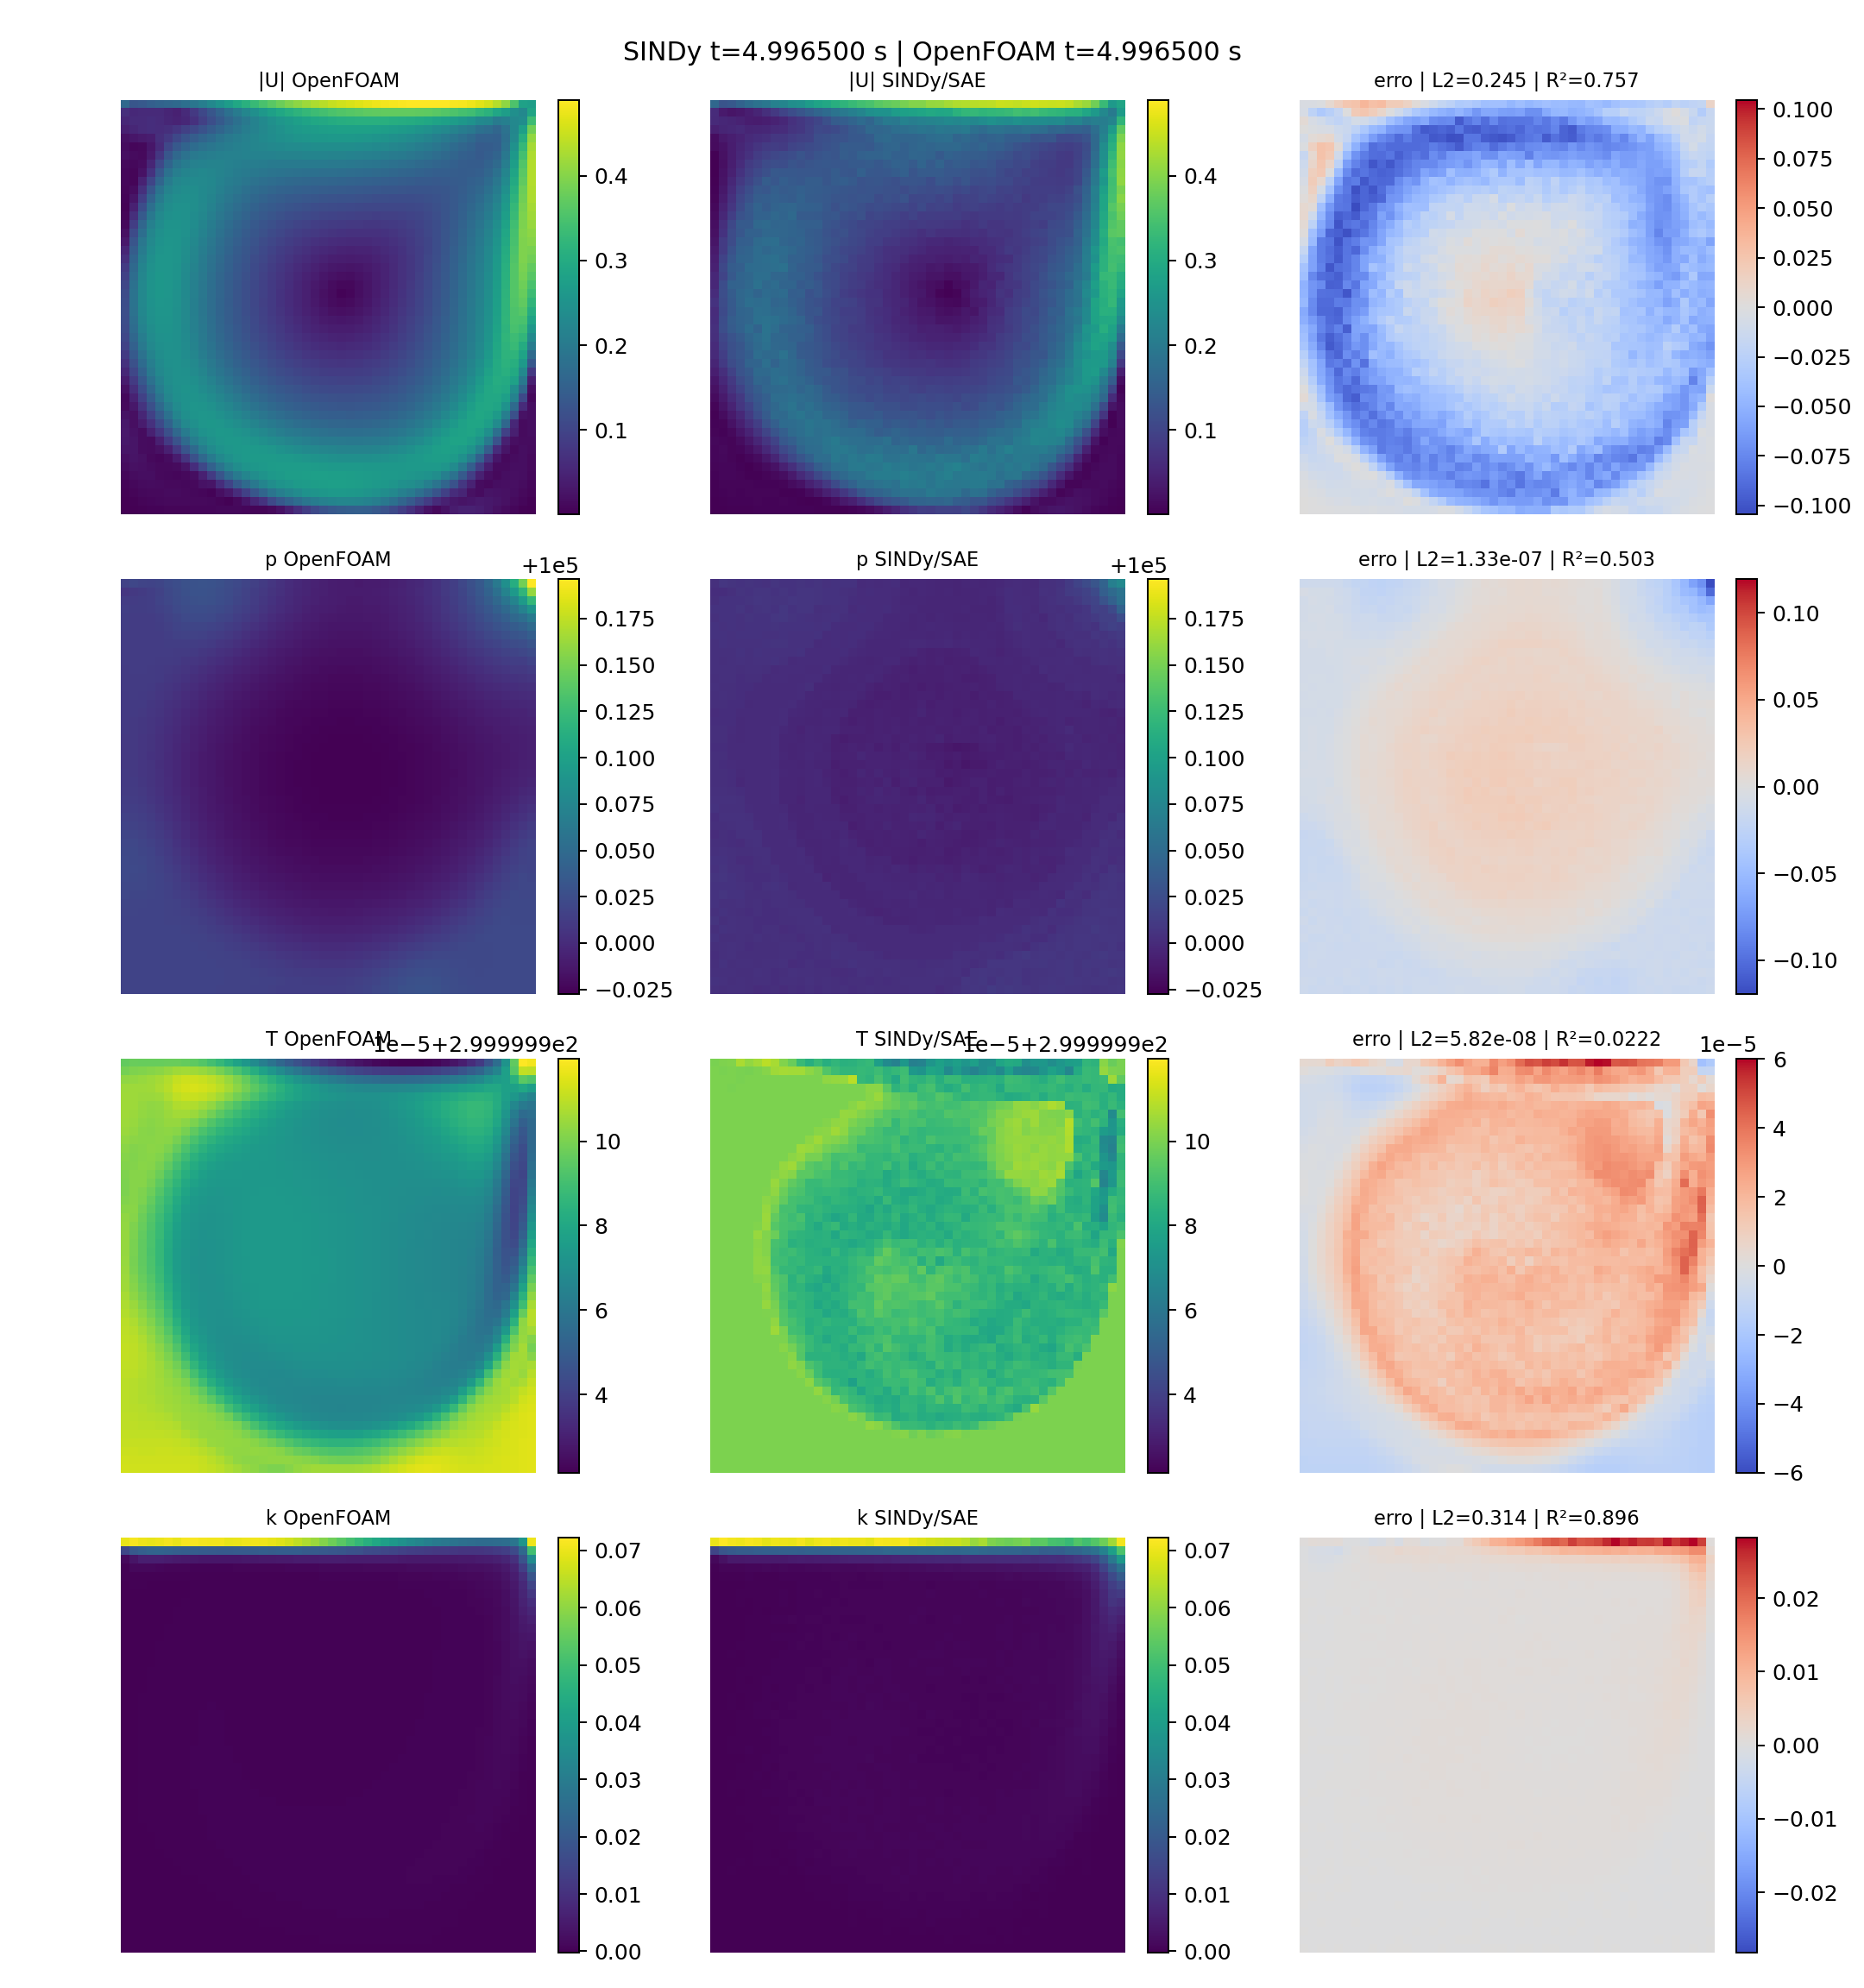
\includegraphics[width=\linewidth]{cavity_direto.png}\caption{Cavity em $t=4,9965$ s.}\end{subfigure}
\caption{Validação de campos nos casos mais desafiadores.}\end{figure}

\subsection{Auditoria da cavidade e validação corrigida}
A POD legada da cavity continha $\alpha_{water}$ e $p_{rgh}$ nulos. O resultado não havia sido copiado pronto: geometria, tempos e $U,k$ eram da cavidade, mas o código era um template de dam-break adaptado parcialmente. A POD corrigida com $U_x,U_y,p,T,k$ atingiu 99,303\% da energia em 8 modos e 99,988\% em 50. O POD--SINDy corrigido reduziu o erro de derivada para 0,0729, mas continuou incapaz de integração livre. Portanto, a inconsistência de campos prejudicava a análise, porém não era a única causa da instabilidade.

A comparação direta OpenFOAM--\allowbreak SAE--\allowbreak POD--\allowbreak SINDy mostrou, em $t=1,25;2,50;3,74;5,00$ s, erro de $|U|$ entre 0,128 e 0,245 e $R^2$ entre 0,757 e 0,958. Para $k$, o erro cresceu de 0,024 para 0,314, com $R^2$ ainda igual a 0,896 no final. Pressão e temperatura mantiveram a média, mas suas flutuações apresentaram $R^2$ baixo. A validação anterior, baseada em índice normalizado até 1 s, foi marcada como inválida.

\subsection{Síntese científica}
Os resultados sustentam quatro conclusões intermediárias. Primeiro, POD e SAE isolados medem capacidade de representação, não previsão. Segundo, a não linearidade do SAE não garante coordenadas dinamicamente simples. Terceiro, a POD latente melhora o condicionamento do SINDy de forma consistente, mas não elimina erro acumulado. Quarto, rastreabilidade de campos, tempos e artefatos é tão importante quanto a escolha do algoritmo: métricas numericamente boas podem ser produzidas por canais nulos, médias dominantes ou validações guiadas.

\novasecao{CONCLUSÃO}
Em relação ao plano aprovado, foram concluídos a revisão bibliográfica, o treinamento no OpenFOAM e em bibliotecas Python, a geração e organização de dados em geometrias simplificadas, o desenvolvimento e a avaliação de POD/SAE, a identificação por SINDy, a interpretação comparativa e a divulgação científica. A progressão do relatório parcial ao artigo do CBCFD e, depois, aos quatro estudos finais evidencia a passagem de aprendizado e reconstrução para descoberta e validação dinâmica.

O objetivo de comparar modelos reduzidos foi atingido e ampliado. A POD mostrou-se uma referência robusta de compressão linear. O SAE capturou relações não lineares, mas sua generalização variou fortemente e não superou sistematicamente a POD. Os SINDy diretos apresentaram instabilidade em integração livre, demonstrando que ajuste local não comprova captura da dinâmica. O SAE--POD--SINDy foi a arquitetura mais robusta: todos os modelos selecionados completaram o intervalo, enquanto os SAE--SINDy falharam. O melhor resultado foi o dam-break URANS, com erro livre 0,551 e $R^2=0,697$; ainda assim, nenhum caso alcançou precisão suficiente para substituir a simulação de alta fidelidade sem ressalvas.

A hipótese de que a POD estabiliza o espaço latente foi confirmada qualitativamente. A transformação reduz correlação e direções ruidosas, favorecendo a regressão e a integração. Entretanto, quando há truncamento, o efeito mistura condicionamento e perda de informação. A relação com a modelagem ambiental permanece metodológica: os casos estudados representam bancos de prova controlados para técnicas que poderão ser transferidas a escoamentos atmosféricos, oceânicos ou de transporte, mas não constituem ainda uma simulação ambiental real.

Duas metas previstas permaneceram parciais: a análise paramétrica foi limitada à comparação entre laminar, URANS e LES, sem varredura sistemática, e as equações reduzidas não foram implementadas como um novo modelo no OpenFOAM. Também faltou realizar ajustes mais amplos nas arquiteturas e nos hiperparâmetros, incluindo profundidade e largura do autoencoder, dimensão e regularização do espaço latente, taxa de aprendizado, biblioteca de funções, limiares de esparsidade e parâmetros de integração do SINDy. Embora esses ajustes sejam necessários para buscar maior generalização e estabilidade, não foi possível concluir uma varredura abrangente dentro do período e dos recursos computacionais disponíveis.

A continuidade será realizada sobre os escoamentos microfluídicos controlados por microválvulas Tesla de Vieira \cite{vieira2025}. Após validar malha, convergência e condições equivalentes nos sentidos direto e reverso, serão formados bancos de snapshots de velocidade e pressão para aplicar POD, SAE e SINDy. Pretende-se avaliar variações de número de Reynolds e geometria, relacionar as coordenadas reduzidas a vórtices, perda de carga e diodicidade e investigar modelos condicionados pela direção do fluxo. Paralelamente, deverão ser comparadas POD equidimensional e truncada, regularidade temporal do SAE, seleção da biblioteca SINDy por integração livre e inclusão de restrições físicas.

\novasecao{DIFICULDADES ENCONTRADAS}
As principais dificuldades e ações corretivas foram:
\begin{enumerate}
\item \textbf{Alto custo e volume de dados.} Matrizes com até 10001 snapshots provocaram risco de falta de memória. Foram usados subamostragem, memmap e SVD aleatorizada truncada na correção da cavity.
\item \textbf{Generalização do SAE.} Taxa de aprendizado baixa, poucos snapshots e compressão excessiva prejudicaram o LES. A configuração foi alterada para 1001 snapshots, 32 latentes e taxa $10^{-3}$, melhorando treino, embora a validação ainda seja limitada.
\item \textbf{Instabilidade do SINDy.} Integrações falharam por rigidez, biblioteca densa e coordenadas mal condicionadas. Foram testados Lasso/Adalasso, suavização, ordens diferentes e POD latente.
\item \textbf{Proveniência.} Notebooks atuais e modelos salvos nem sempre correspondem. Os relatórios distinguem configuração declarada, artefato executado e reexecução corrigida.
\end{enumerate}

A divulgação científica ocorreu em etapas. O artigo do CBCFD apresentou apenas POD e SAE da prova de conceito da cavity, coerentemente com o estágio alcançado naquele momento, e anunciou SINDy como continuidade. A identificação dinâmica e a auditoria de dados foram desenvolvidas depois e, por isso, devem originar publicação posterior específica, sem alterar retrospectivamente o escopo do artigo já publicado.

\novasecao{REFERÊNCIAS BIBLIOGRÁFICAS}
\begin{thebibliography}{99}\setlength{\itemsep}{0.6em}
\bibitem{brunton2016} BRUNTON, S. L.; PROCTOR, J. L.; KUTZ, J. N. Discovering governing equations from data by sparse identification of nonlinear dynamical systems. \textit{Proceedings of the National Academy of Sciences}, v. 113, n. 15, p. 3932--3937, 2016.
\bibitem{hinton2006} HINTON, G. E.; SALAKHUTDINOV, R. R. Reducing the dimensionality of data with neural networks. \textit{Science}, v. 313, n. 5786, p. 504--507, 2006.
\bibitem{hirt1981} HIRT, C. W.; NICHOLS, B. D. Volume of Fluid method for the dynamics of free boundaries. \textit{Journal of Computational Physics}, v. 39, p. 201--225, 1981.
\bibitem{lin2024} LIN, X.; XIAO, D.; FANG, F. Data discovery of low dimensional fluid dynamics of turbulent flows. \textit{arXiv preprint arXiv:2401.05449}, 2024. Disponível em: \url{https://arxiv.org/abs/2401.05449}. Acesso em: 28 set. 2026.
\bibitem{menter1994} MENTER, F. R. Two-equation eddy-viscosity turbulence models for engineering applications. \textit{AIAA Journal}, v. 32, n. 8, p. 1598--1605, 1994.
\bibitem{nicoud1999} NICOUD, F.; DUCROS, F. Subgrid-scale stress modelling based on the square of the velocity gradient tensor. \textit{Flow, Turbulence and Combustion}, v. 62, p. 183--200, 1999.
\bibitem{openfoam} OPENFOAM FOUNDATION. \textit{OpenFOAM version 13: user guide and source documentation}. 2025. Disponível em: \url{https://openfoam.org}. Acesso em: 28 set. 2026.
\bibitem{sirovich1987} SIROVICH, L. Turbulence and the dynamics of coherent structures. I--III. \textit{Quarterly of Applied Mathematics}, v. 45, n. 3, p. 561--590, 1987.
\bibitem{vieira2025} VIEIRA, B. M. M. \textit{Modelagem computacional de escoamentos microfluídicos controlados por microválvulas Tesla}. Relatório Final de Iniciação Científica, Universidade Federal de Mato Grosso, Cuiabá, 2025.
\end{thebibliography}

\novasecao{PRODUTOS GERADOS}
Os produtos refletem as etapas sucessivas do plano:
\begin{enumerate}
\item \textbf{Relatório parcial de iniciação científica}, referente a 30/10/2025--28/02/2026, com revisão, tutoriais OpenFOAM e resultados iniciais de POD/SAE em cavity e damBreakLaminarFine;
\item \textbf{artigo publicado no congresso CBCFD}: CHAGAS JUNIOR, Eldo Francisco; MAIONCHI, Daniela de Oliveira. \textit{Redução de dimensionalidade em escoamento cavity via POD e SAE a partir de dados do OpenFOAM}. Trabalho de quatro páginas sobre a etapa de 1001 snapshots de velocidade;
\item quatro relatórios técnicos em LaTeX/PDF: dam-break laminar, dam-break URANS, dam-break LES--WALE e cavity URANS;
\item este relatório final consolidado, alinhado ao projeto, ao relatório parcial, ao artigo e ao modelo institucional da UFMT;
\item casos e dados OpenFOAM, notebooks e rotinas de POD, SAE, POD--SINDy, SAE--SINDy e SAE--POD--SINDy;
\item arquivos reprodutíveis com equações descobertas, métricas JSON/CSV/NPZ e figuras de comparação;
\item POD corrigida da cavity com $U_x,U_y,p,T,k$, rejeição explícita de snapshots incompletos e SVD truncada eficiente;
\item validador direto OpenFOAM--SINDy com alinhamento por tempo físico e documentação das inconsistências, artefatos legados e ações corretivas.
\end{enumerate}

\noindent O arquivo disponibilizado do artigo não informa no texto extraído edição, local, páginas dos anais, DOI ou URL pública do CBCFD. Esses dados bibliográficos devem ser acrescentados à versão de submissão institucional caso constem no certificado ou nos anais do evento.

\end{document}
